% !TEX root = ../rawlik-phd-thesis.tex
\chapter{Next generation active magnetic field compensation}
\label{ch:sfc-prototype}

The coil design method described in the previous chapter opened the door to a next generation of active magnetic field compensation systems. Ones where the coil system is not much larger than the fiducial volume and where high-order terms of the magnetic field can be compensated, all while retaining a low number of controlled degrees of freedom.

% The large fiducial volume is of particular importance for the n2EDM experiment at PSI. The available area\ldots

In the laboratory at ETH Zürich an active magnetic field compensation system was constructed, based on the coil design. The goal was do demonstrate the feasibility of construction of the coils, develop and test the electronic and software parts of the feedback algorithm, and test system as the whole.

\note{Schwammig, work on it!}


\section{The first iteration -- coil structure}
When discussing the coil design method we have already indicated a possible way to realise it in practice---construct a grid out of cable channels. The system, pictured in Fig.\,\ref{fig:prototype_photo}, was built as $5 \times 9 \times 5$ grid of square tiles. Each tile had side length \SI{262}{\milli\meter}, the total size was $1310 \times 1310 \times \SI{2358}{\milli\meter}$. The vertical axis we refer to as $z$, the long horizontal one as $y$, and the remaining as $x$.

\begin{figure}
  \centering
  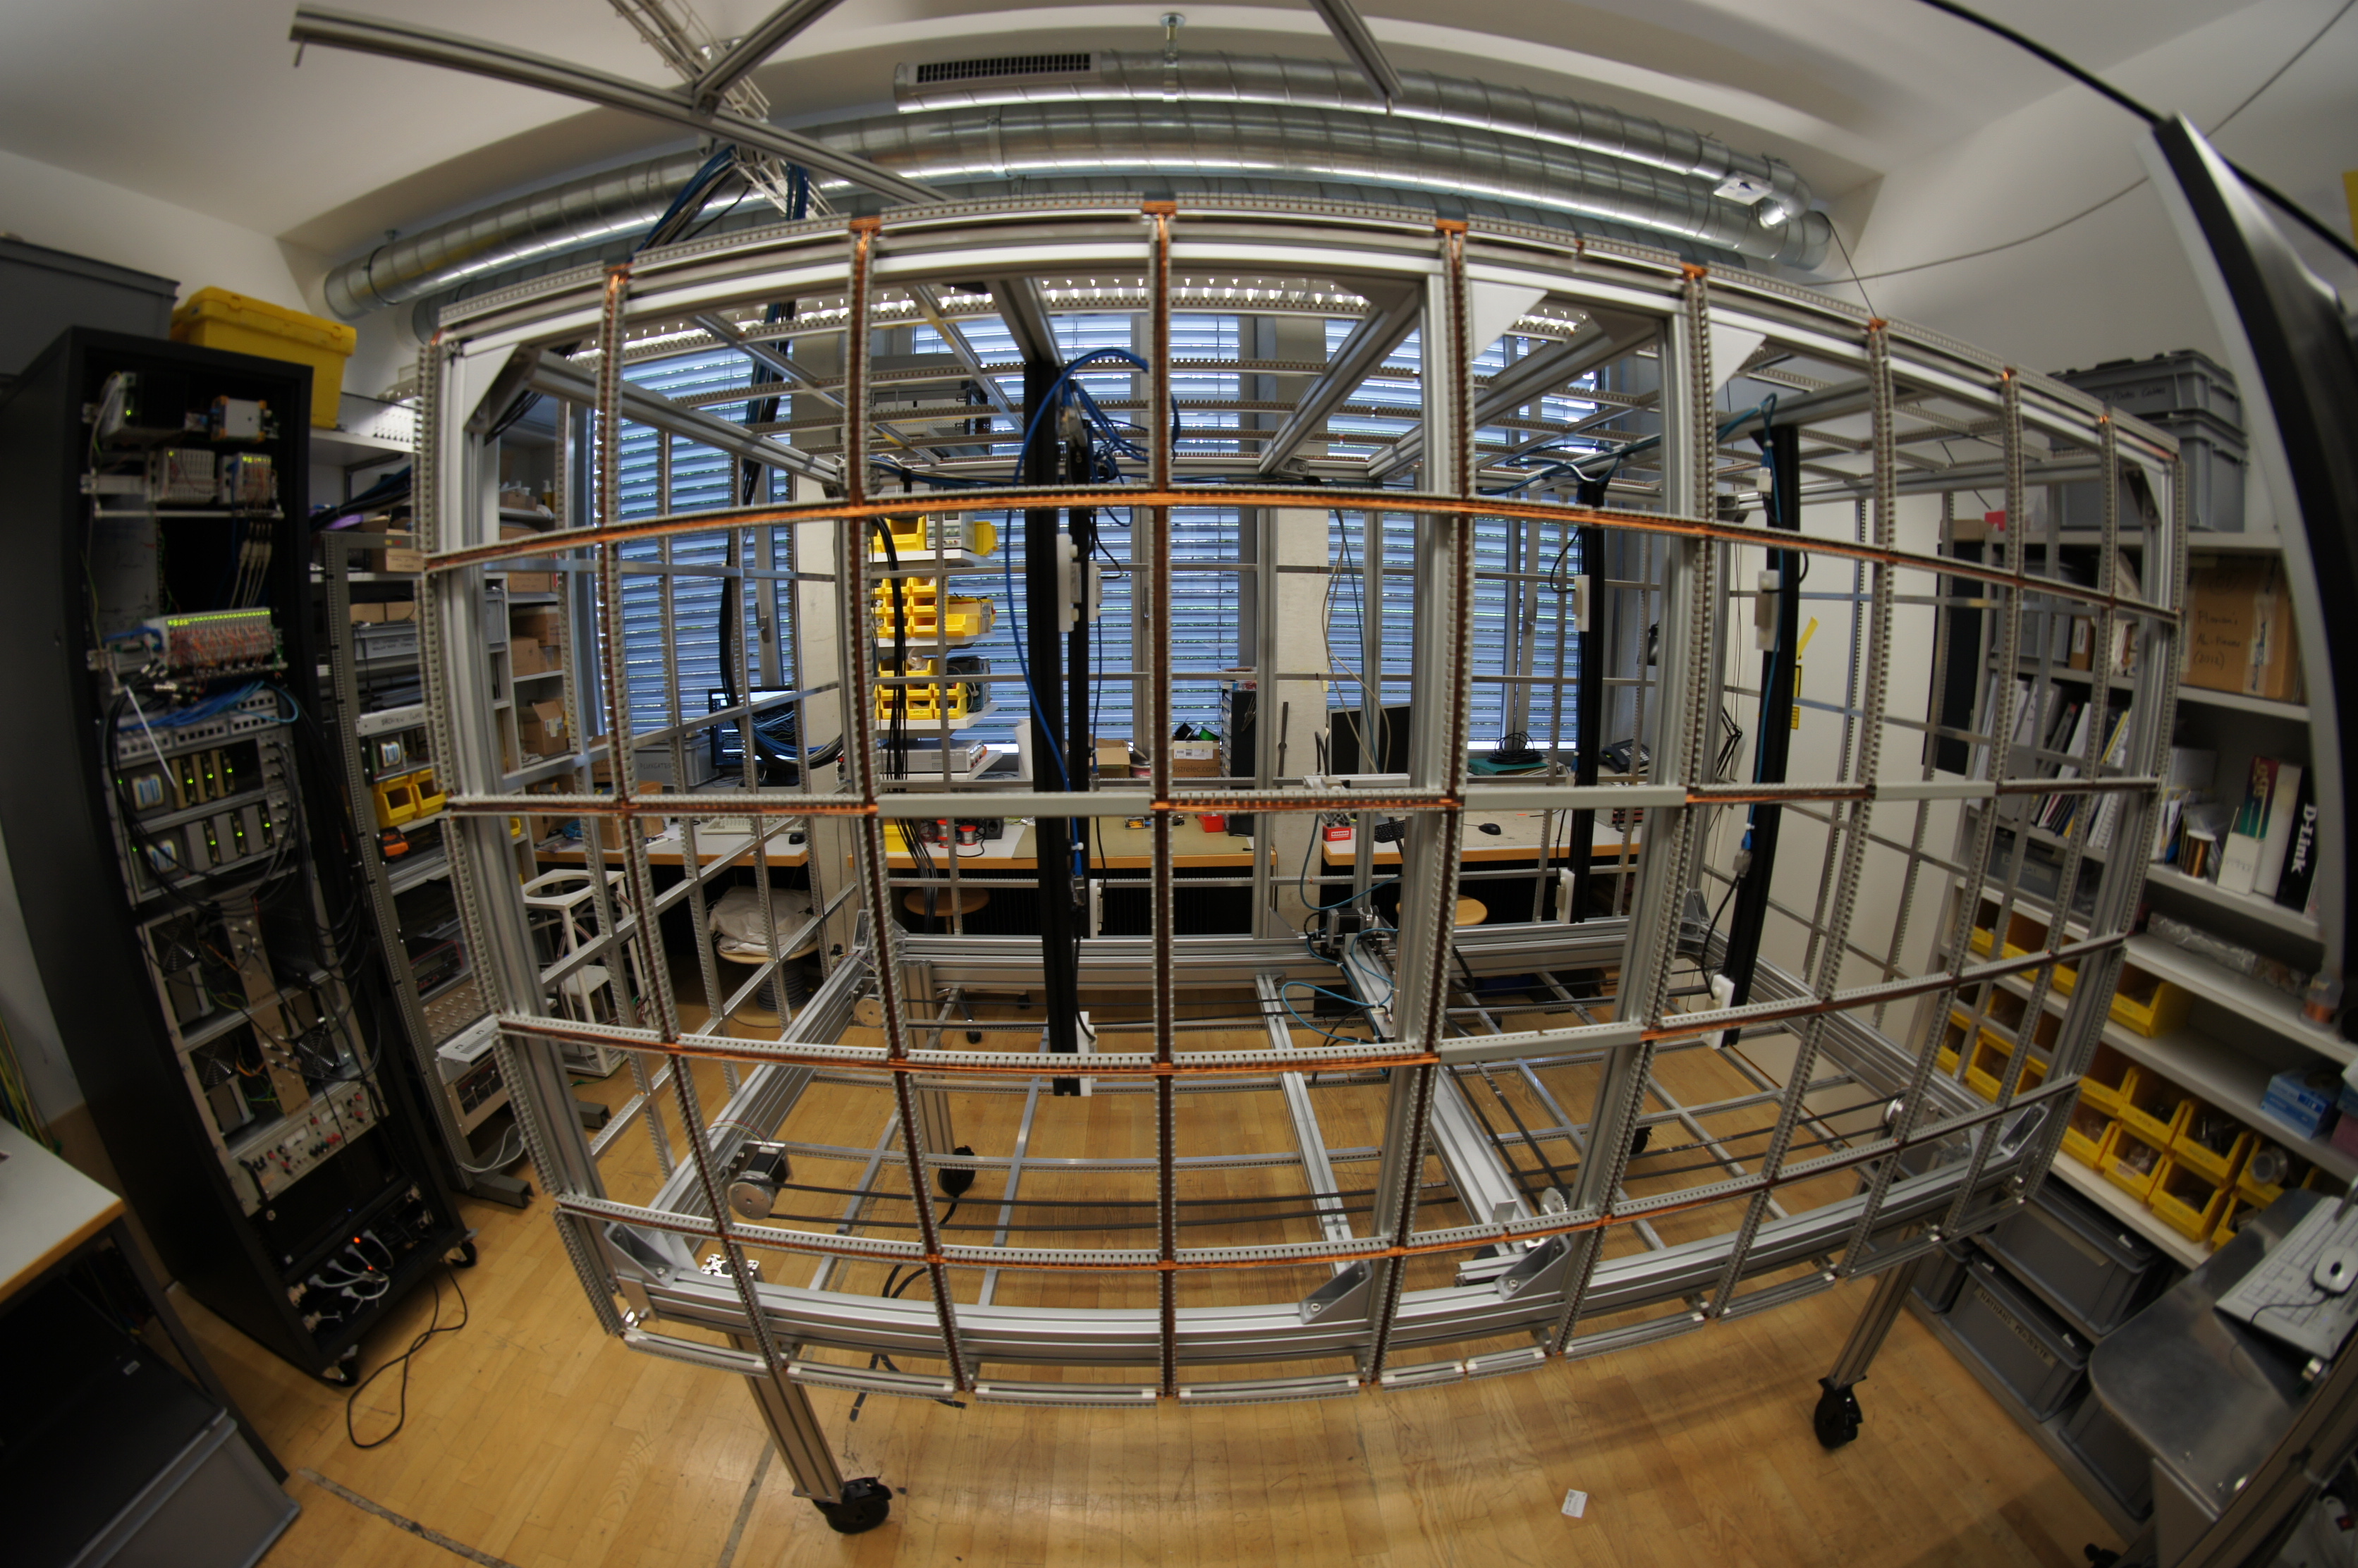
\includegraphics[width=0.9\linewidth]{gfx/prototype/DSC03472.JPG}
  \caption{The active magnetic compensation system in the laboratory at ETH Zürich. It consists cable channels mounted on an aluminum support structure. In the channels copper wires making up the coils can be seen. On the left-hand side the control cabinet of the system is visible.}
  \label{fig:prototype_photo}
\end{figure}

The support frame was made of aluminum construction profiles. To support the cable channels, on each side there was a large, one-piece aluminum sheet with square cut-outs leaving the material only directly below the cable channels. The plastic cable channels were glued onto the aluminum.

In its first version the system featured three coils for the homogeneous components of the magnetic field. The coils were designed following the method described in the previous chapter, but excluding the not ready at the time simplification algorithm. The simplification was carried out manually, instead.

\begin{figure}
  \centering
  % 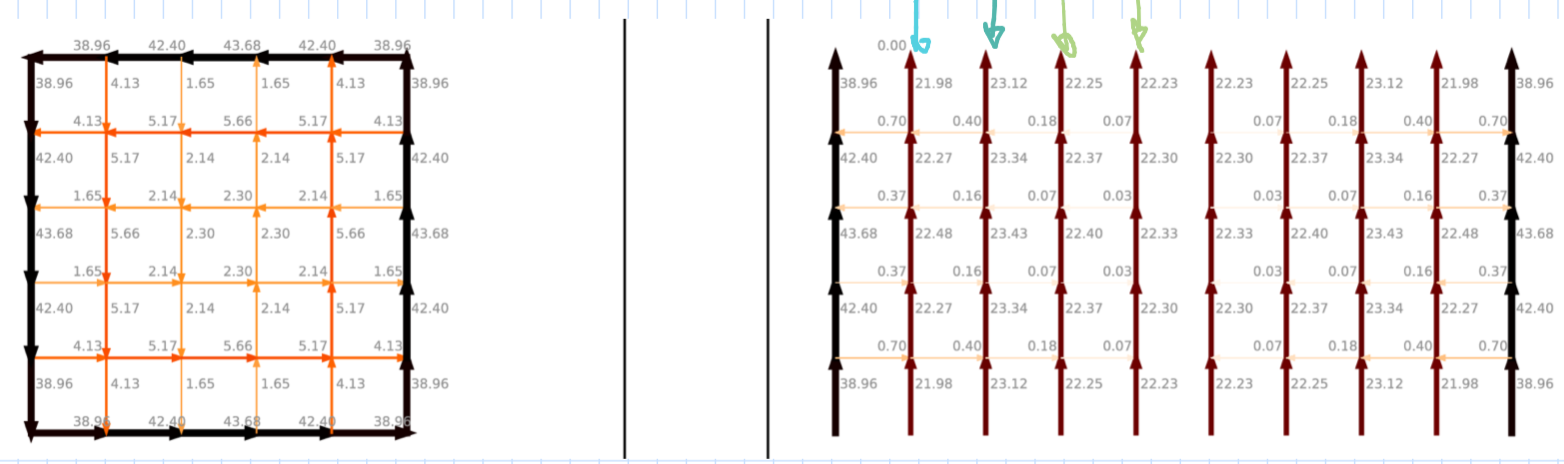
\includegraphics[width=0.9\linewidth]{gfx/prototype/coil_y_currents.png}
  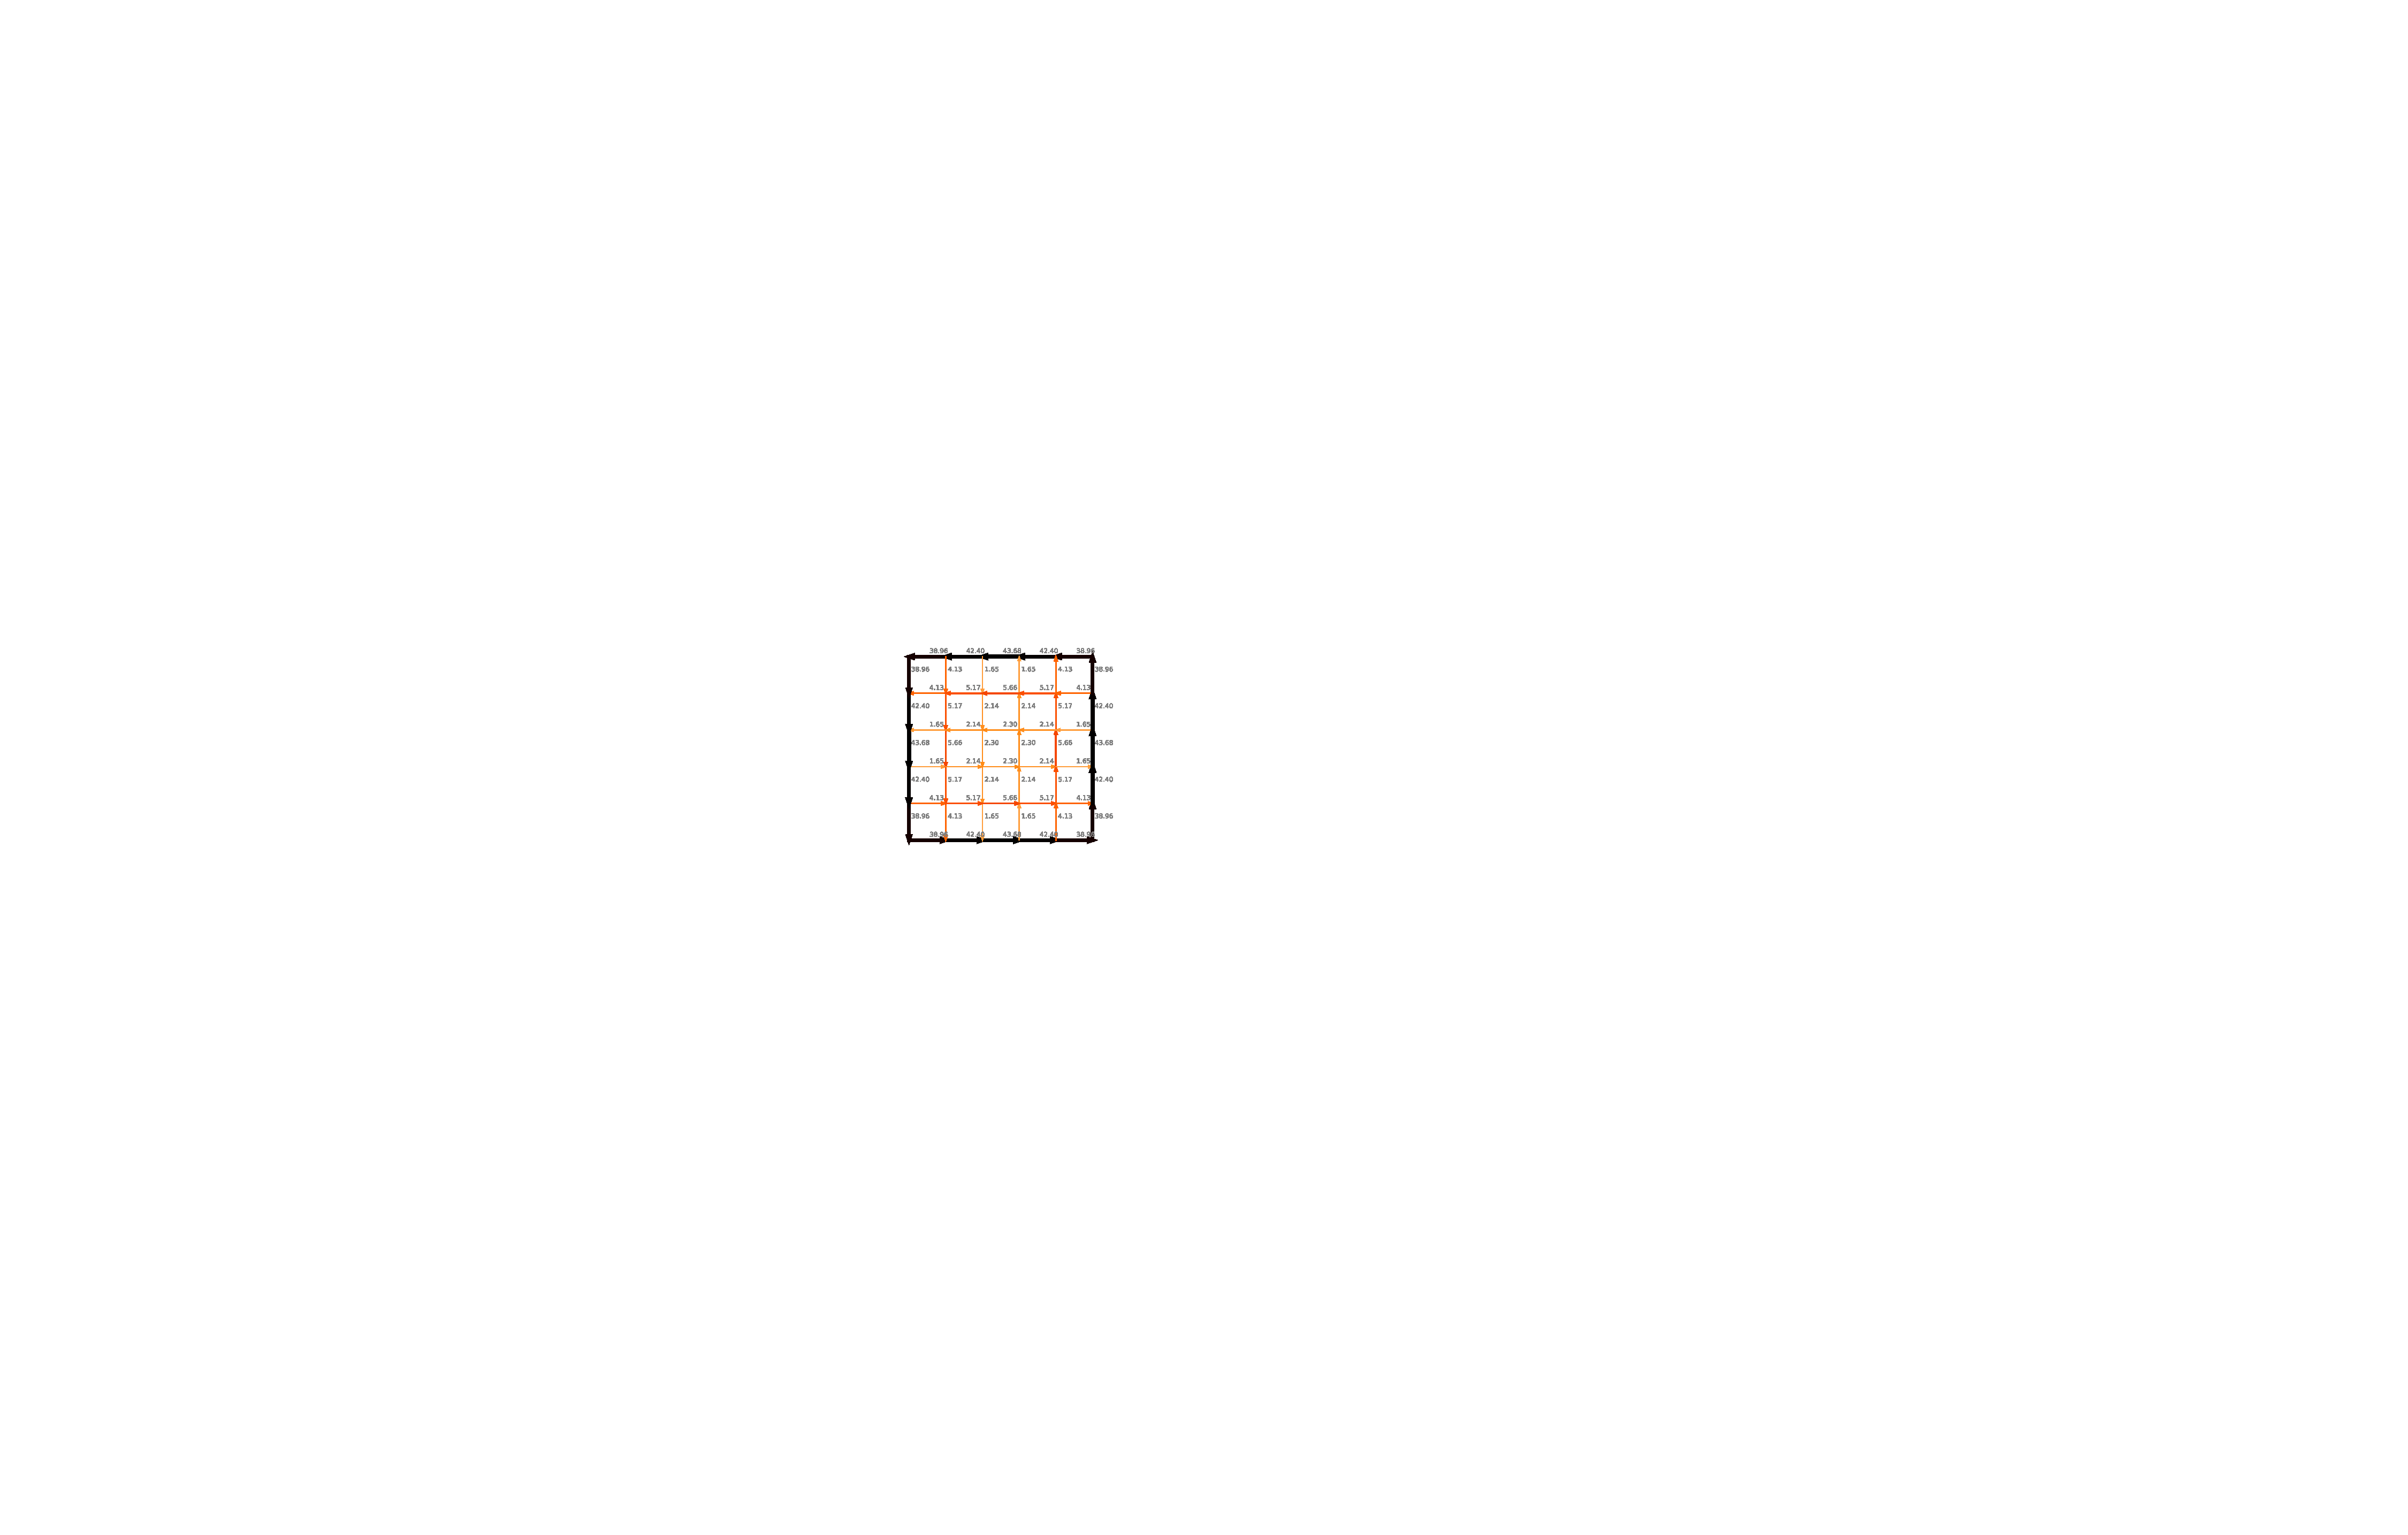
\includegraphics[height=0.3\linewidth]{gfx/prototype/coil_design_y_100uT_1.pdf}
  \quad\quad
  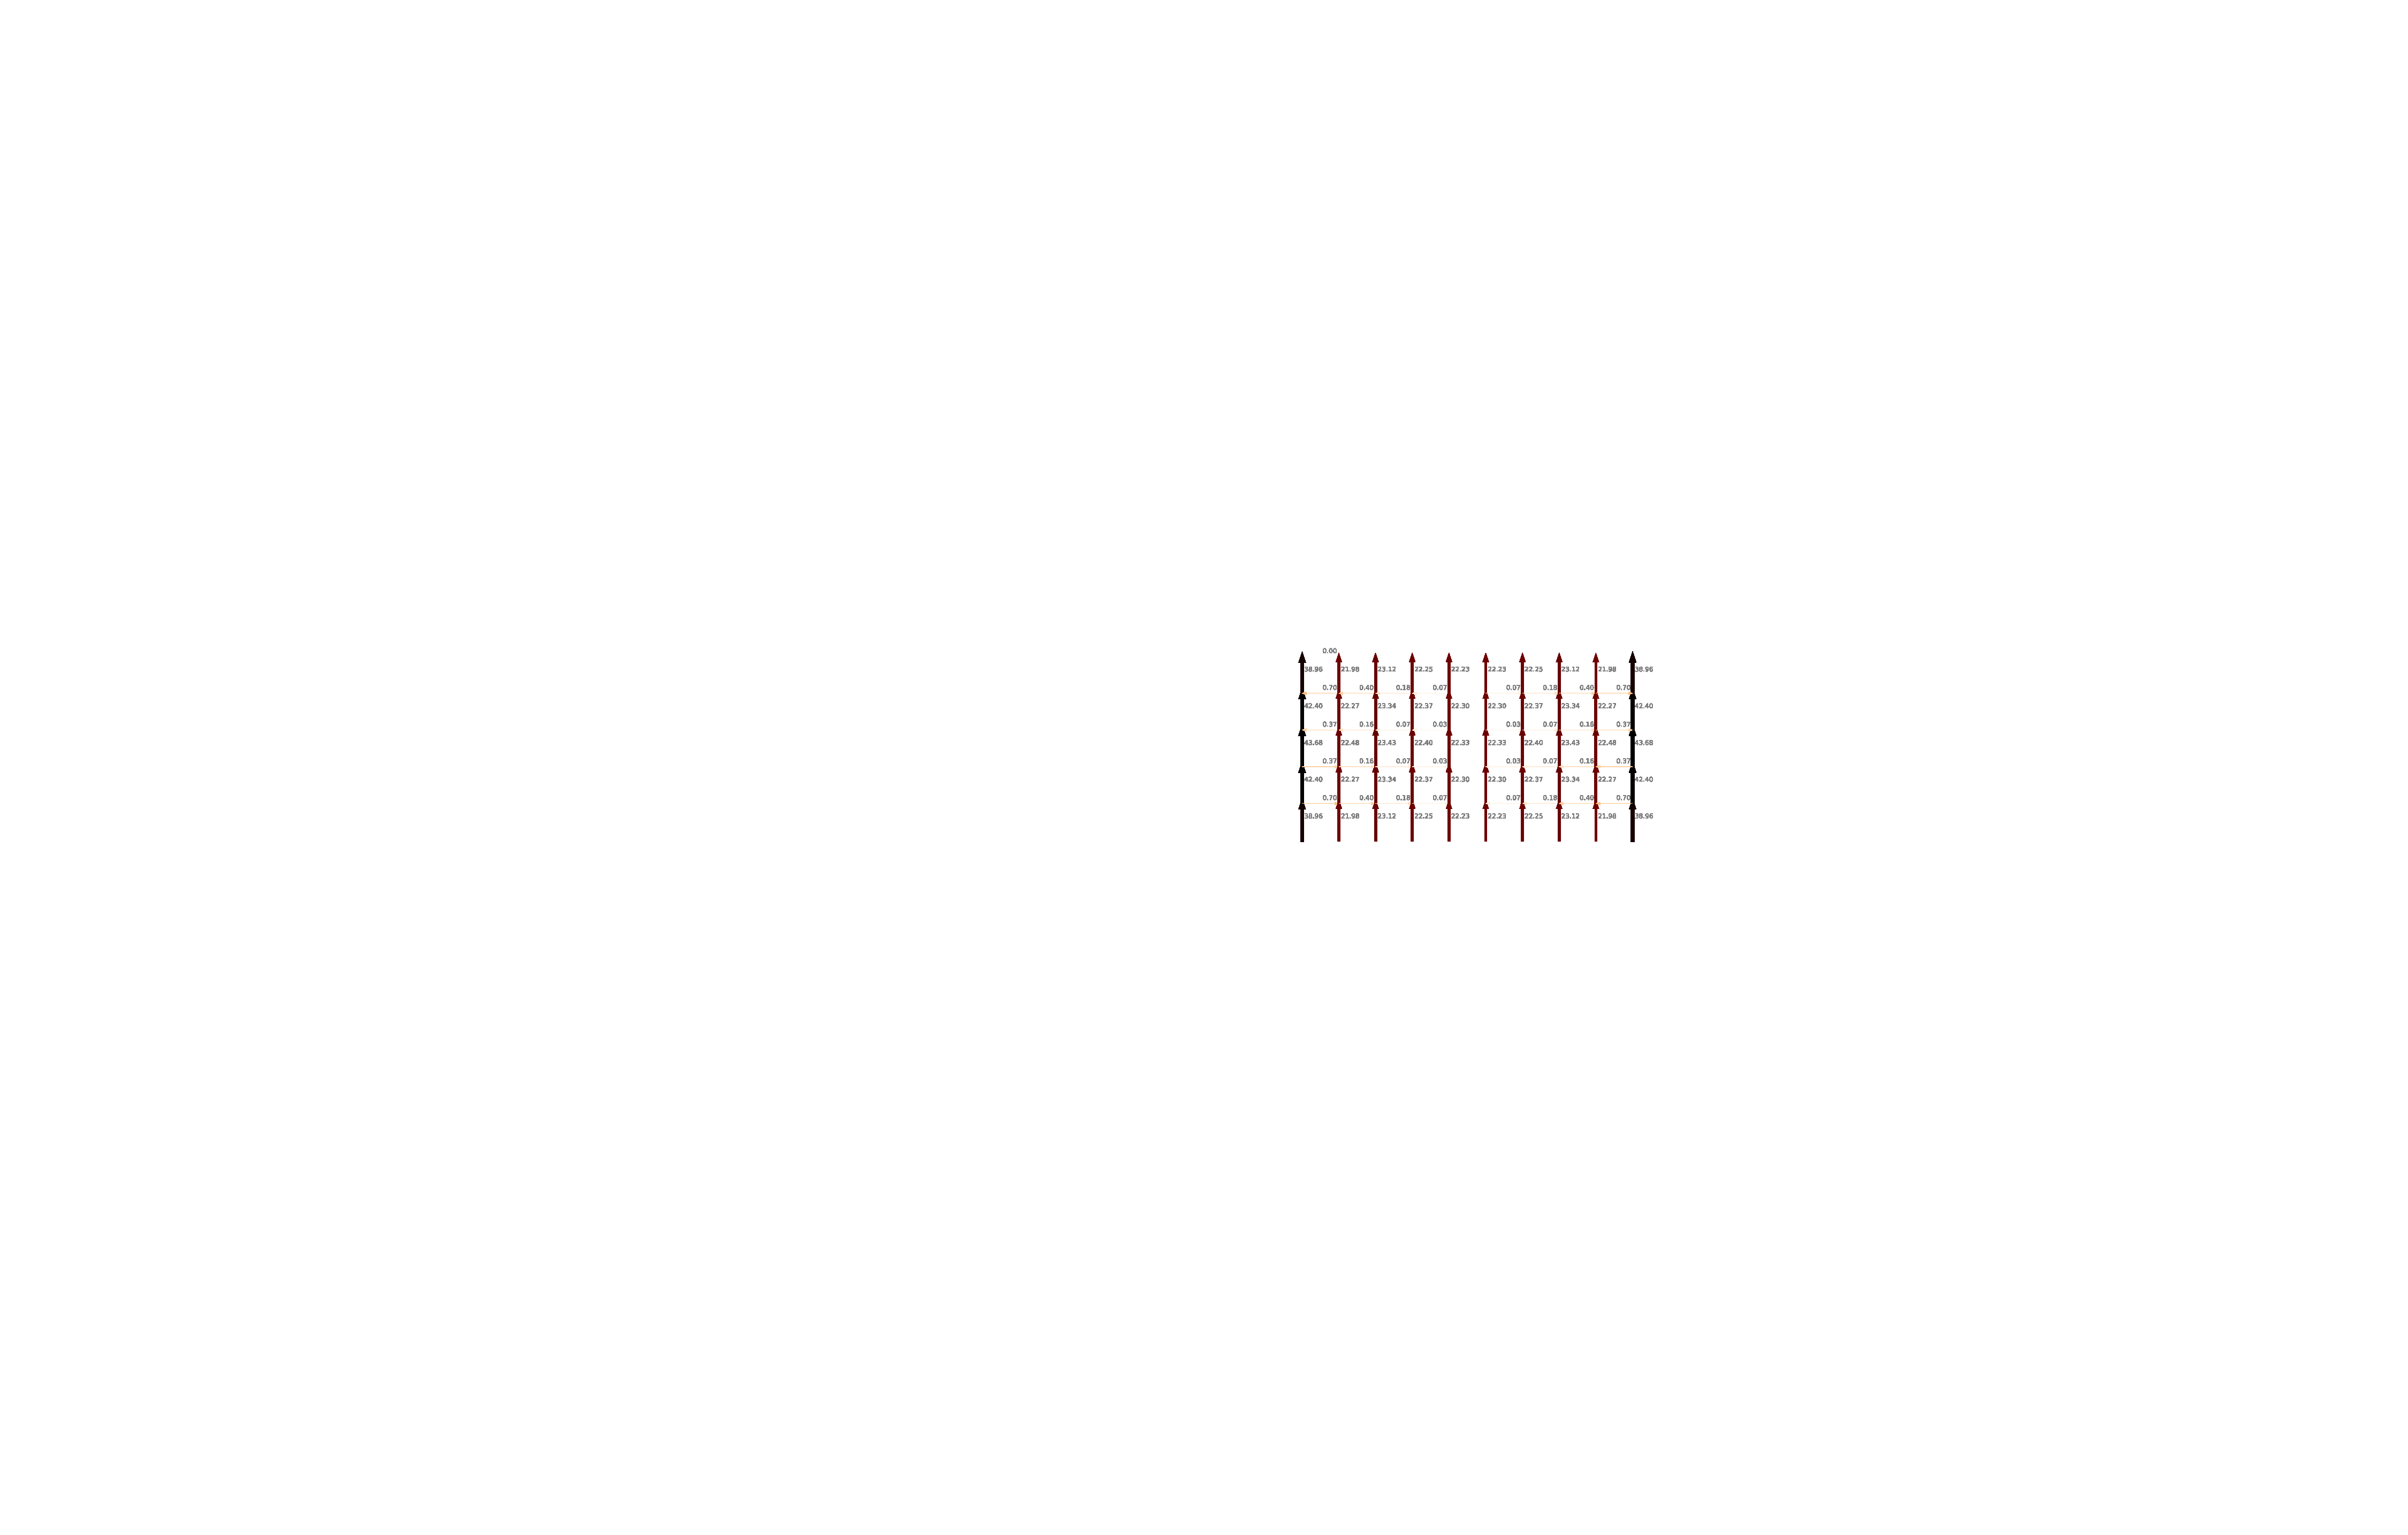
\includegraphics[height=0.3\linewidth]{gfx/prototype/coil_design_y_100uT_2.pdf}
  \caption{The optimal current net for the $y$-coil of the ETH active magnetic field compensation system. Both $5 \times 5$ faces ($y = \mathrm{const}$ planes) are identical and are depicted on the left-hand side. The rectangular faces are all identical, and are depicted on the right-hand side. For each segment the current per \SI{100}{\micro\tesla} of generated field is indicated upwards and to the right from its centre.}
  \label{fig:prototype_coil_y_currents}
\end{figure}

The fiducial volume was chosen to be a cuboid centred in the system, with each of its face \SI{155}{\milli\meter} away from the surface of the coils. The optimal current net for the $y$-coil (producing a homogeneous field in the $y$ direction) is depicted in Fig.\,\ref{fig:prototype_coil_y_currents}. The manual decomposition into loops is shown in Fig.\,\ref{fig:prototype_coil_y_decomposition}. The other two coils, $x$ and $z$, are identical on the symmetry ground. The current net for those is depicted in Fig.\,\ref{fig:prototype_coil_x_z_currents}
% and the decomposition in Fig.\,\ref{fig:prototype_coil_x_z_decomposition}.

\begin{figure}
  \centering
  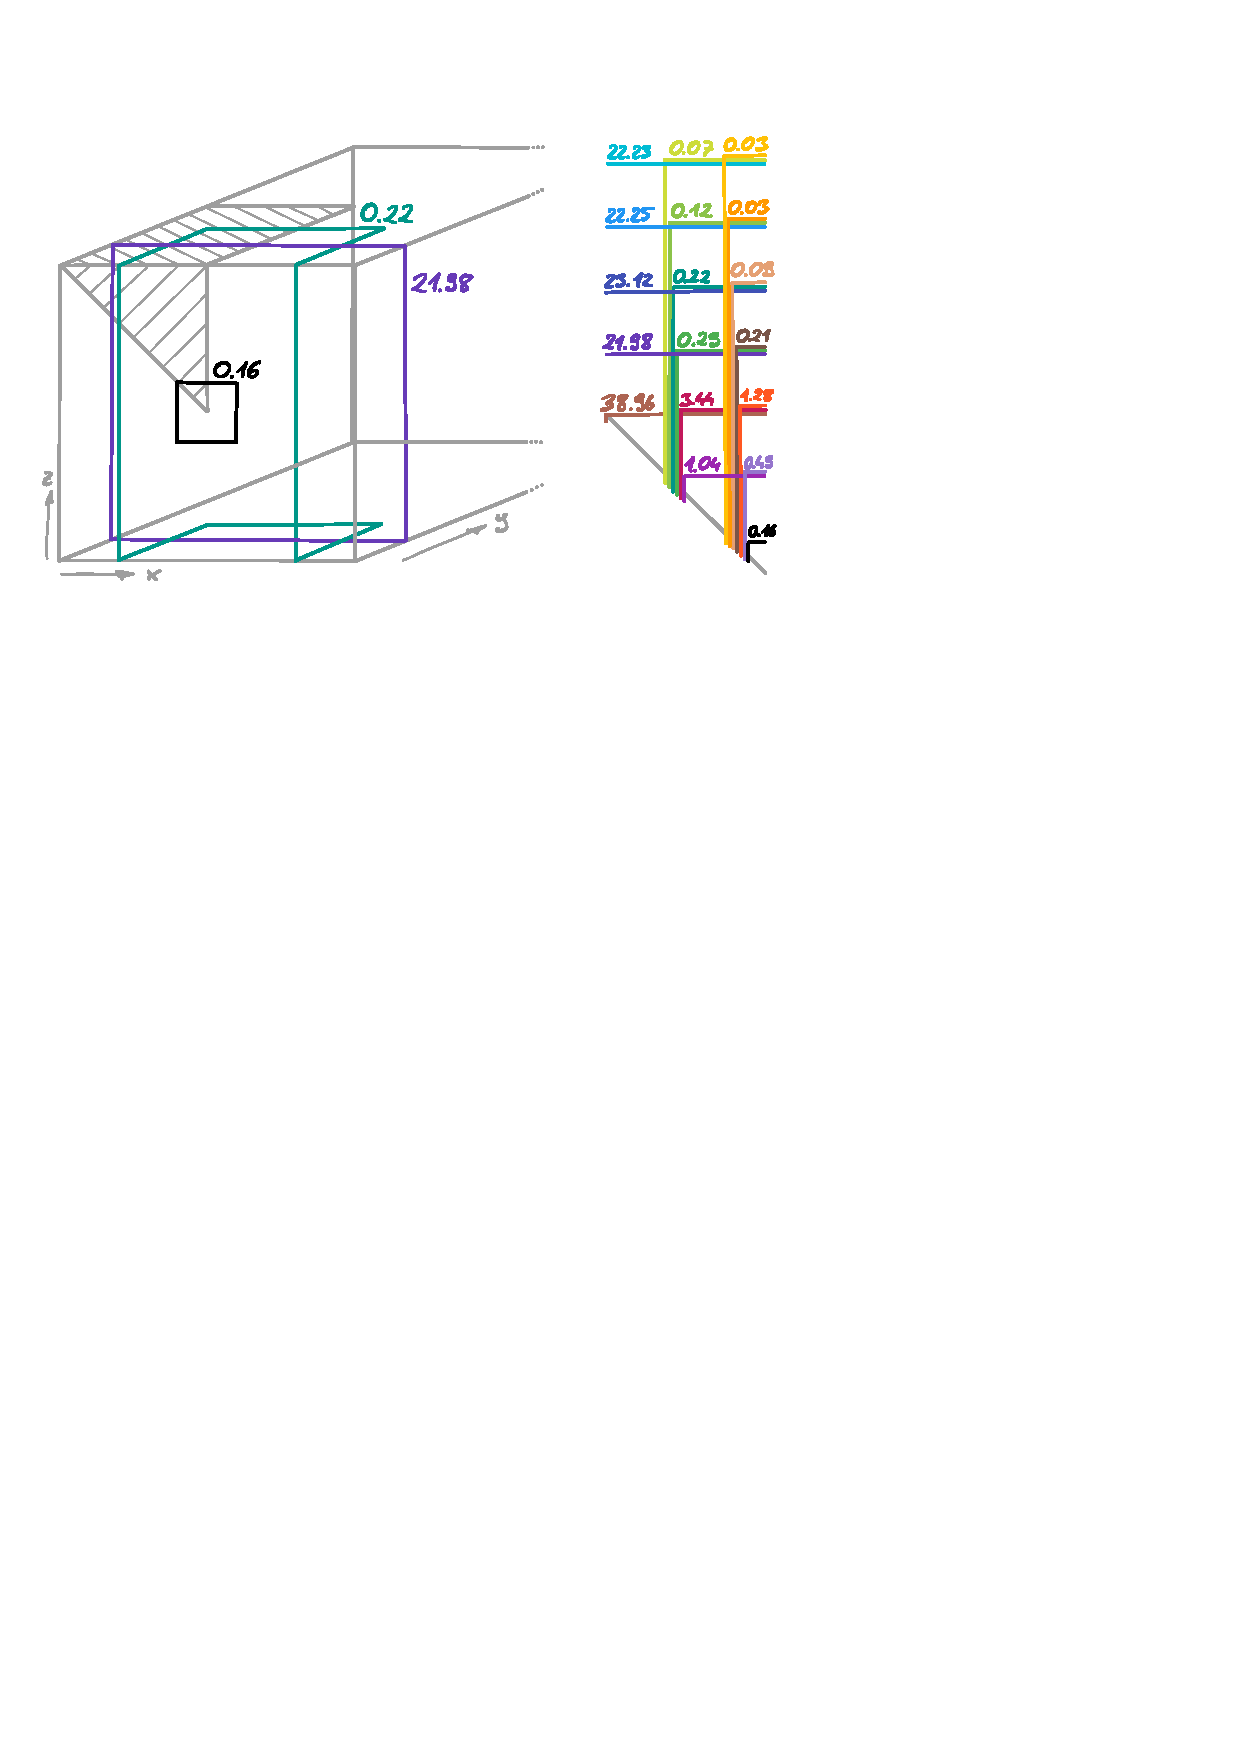
\includegraphics[width=0.9\linewidth]{gfx/prototype/coil_y_decomposition.pdf}
  \caption{The decomposition of the current net of the $y$-coil (Fig.\,\ref{fig:prototype_coil_y_currents}) into current loops. For clarity only a sixteenth part of the system is depicted, all others being identical on the grounds of symmetry. Each loop is indicated with a different colour. The currents are given per \SI{50}{\micro\tesla} of generated field. SHOW WHICH PART IS DEPICTED ON A SMALL 3D DRAWING}
  \label{fig:prototype_coil_y_decomposition}
\end{figure}

\begin{figure}
  \centering
  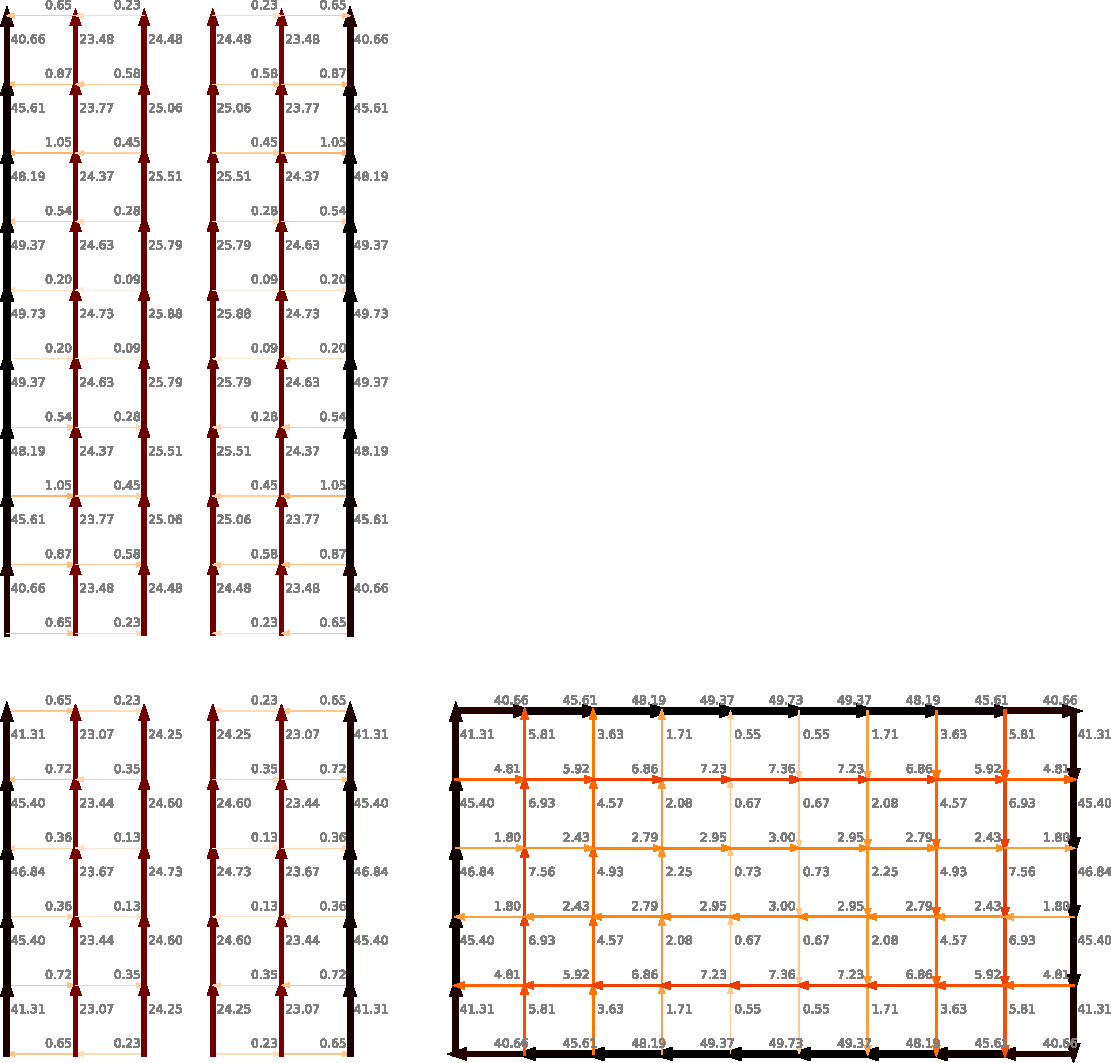
\includegraphics[width=0.9\linewidth]{gfx/prototype/coil_design_x_100uT.pdf}
  \caption{The optimal current net for the $x$ and $z$-coils of the ETH active magnetic field compensation system. Both $5 \times 5$ faces ($y = \mathrm{const}$ planes) are identical and are depicted in the lower-left corner. The rectangular faces perpendicular to the field are depicted to the right, and the ones parallel to it on top. For each segment the current per \SI{100}{\micro\tesla} of generated field is indicated upwards and to the right from its centre.}
  \label{fig:prototype_coil_x_z_currents}
\end{figure}

% up to the point of the simplification algorithm. Here, The decomposition into loops was done by exploiting symmetries of the system. It is suboptimal in the sense, that there are more windings than there could be.

% Then describe how the coils were designed. The optimized current net is shown in Fig\,\ref{fig:prototype_coil_y_currents} (for the y-coil) and \ref{fig:prototype_coil_x_z_currents} (the x- and z-coils).

% It follows the already described coil design method, up to the point of the simplification algorithm. Here, The decomposition into loops was done by exploiting symmetries of the system. It is suboptimal in the sense, that there are more windings than there could be. The decompositions are depicted in Figs.\,\ref{fig:prototype_coil_y_decomposition} (the y-coil) and \ref{fig:prototype_coil_x_z_decomposition} (the x- and z-coils).

% \begin{figure}
%   \centering
%   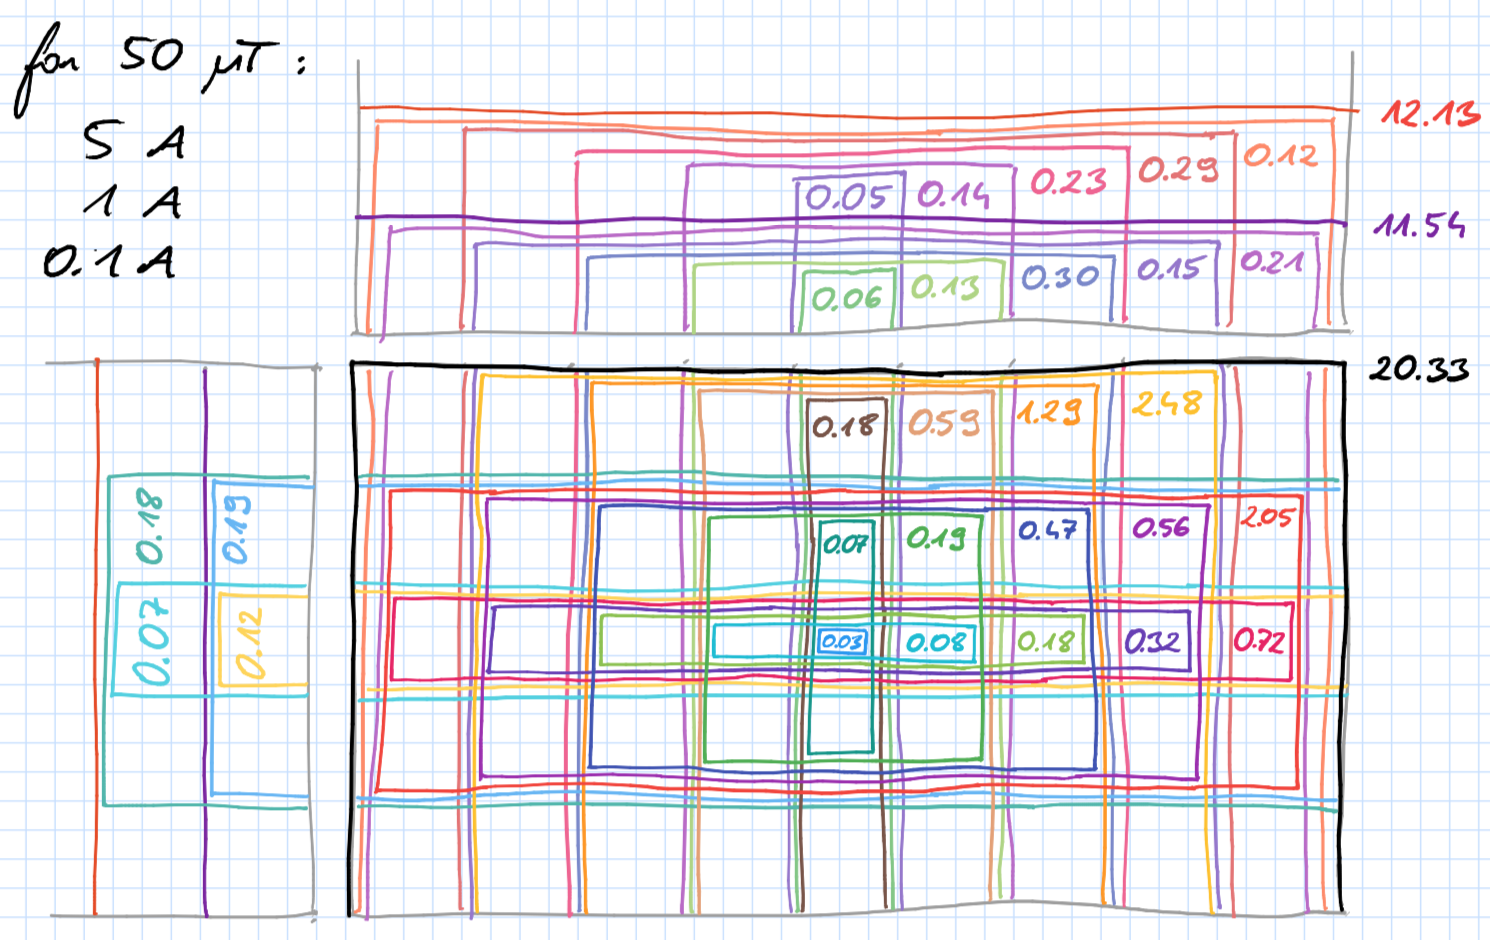
\includegraphics[width=0.9\linewidth]{gfx/prototype/coil_x_z_decomposition.png}
%   \caption{Mention, that it shows\ldots}
%   \label{fig:prototype_coil_x_z_decomposition}
% \end{figure}

Finally, the individual loops were discretised into \SI{10}{\ampere}, \SI{2}{\ampere} and \SI{0.2}{\ampere}, per nominal \SI{100}{\micro\tesla}. For example, the \SI{38.96}{\ampere} current, indicated in black in Fig.\,\ref{fig:prototype_coil_y_decomposition}, was realised as three windings of the \SI{10}{\ampere} wire, four of the \SI{2}{\ampere} one and five of the \SI{0.2}{\ampere} one.

\begin{figure}
  \centering
  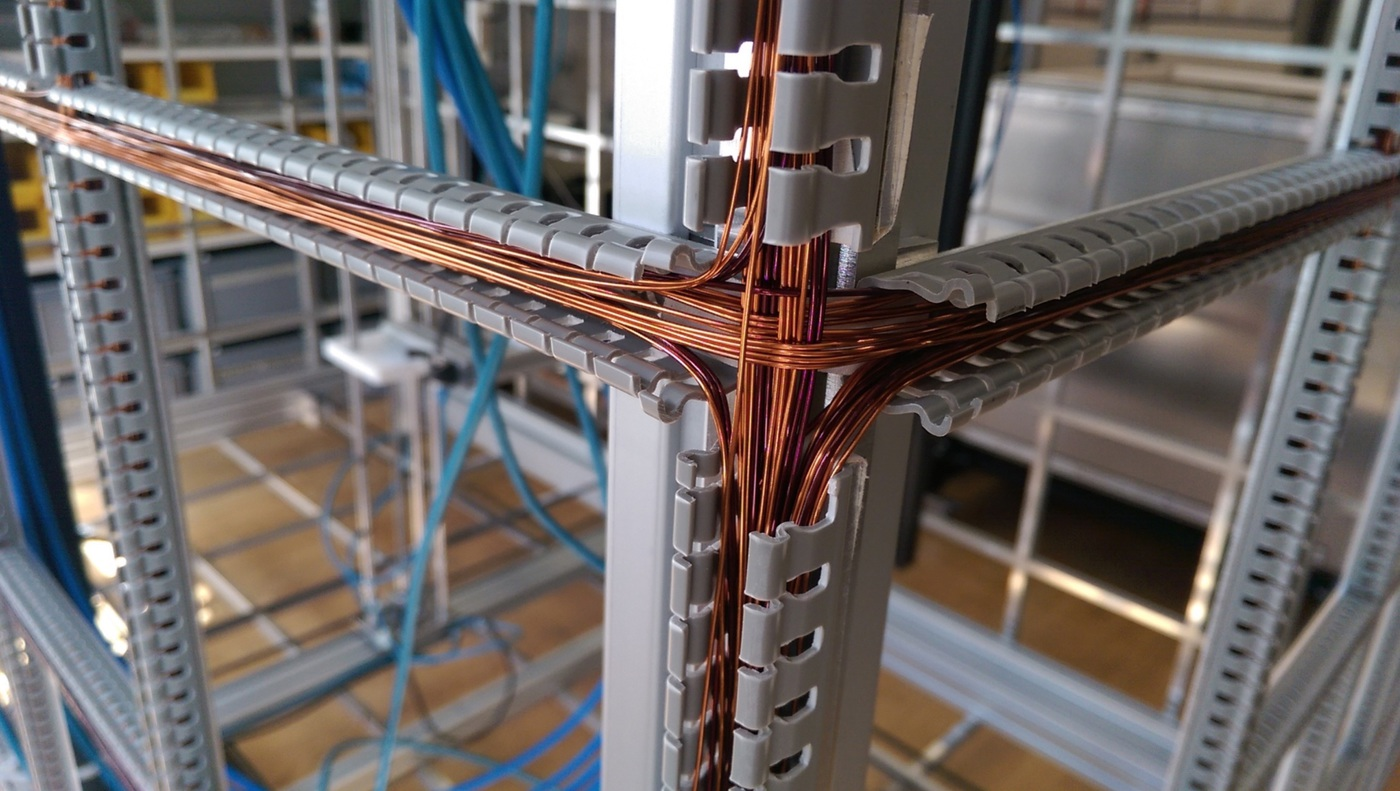
\includegraphics[width=0.9\linewidth]{gfx/prototype/wires_close_up.jpg}
  \caption{A close-up of the wires in the cable channels. Here all three coils for generating the homogeneous fields ($x$, $y$ and $z$) were laid.}
  \label{fig:prototype_coil_wire_close-up}
\end{figure}

An enameled wire was then laid in the cable channels according to the discretised design. For one current component of a coil, e.g.\ \SI{10}{\ampere} in the $x$-coil, a single, long piece of wire was laid, making up all the windings of all loops. For the three coils, each with three components, nine longs wires were laid, in total.
\marginpar{The wire diameter was \SI{1}{\milli\meter} for the \num{10} and \SI{2}{\ampere} wires, and \SI{0.8}{\milli\meter} for the \SI{0.2}{\ampere} one. The wires were prolonged, when needed.}
A close-up of the wires in the cable channels, for all three coils, is shown in Fig.\,\ref{fig:prototype_coil_wire_close-up}.




\section{Mapping}
The coils were mapped in order to verify that the coils really produce a field of the required homogeneity. For that purpose a robot has been built---a fluxgate on an xyz-table, controlled with stepper motors. The robot, called \emph{mapper}, is pictured in Fig.\,\ref{fig:prototype_photo_inside}.

\begin{figure}
  \centering
  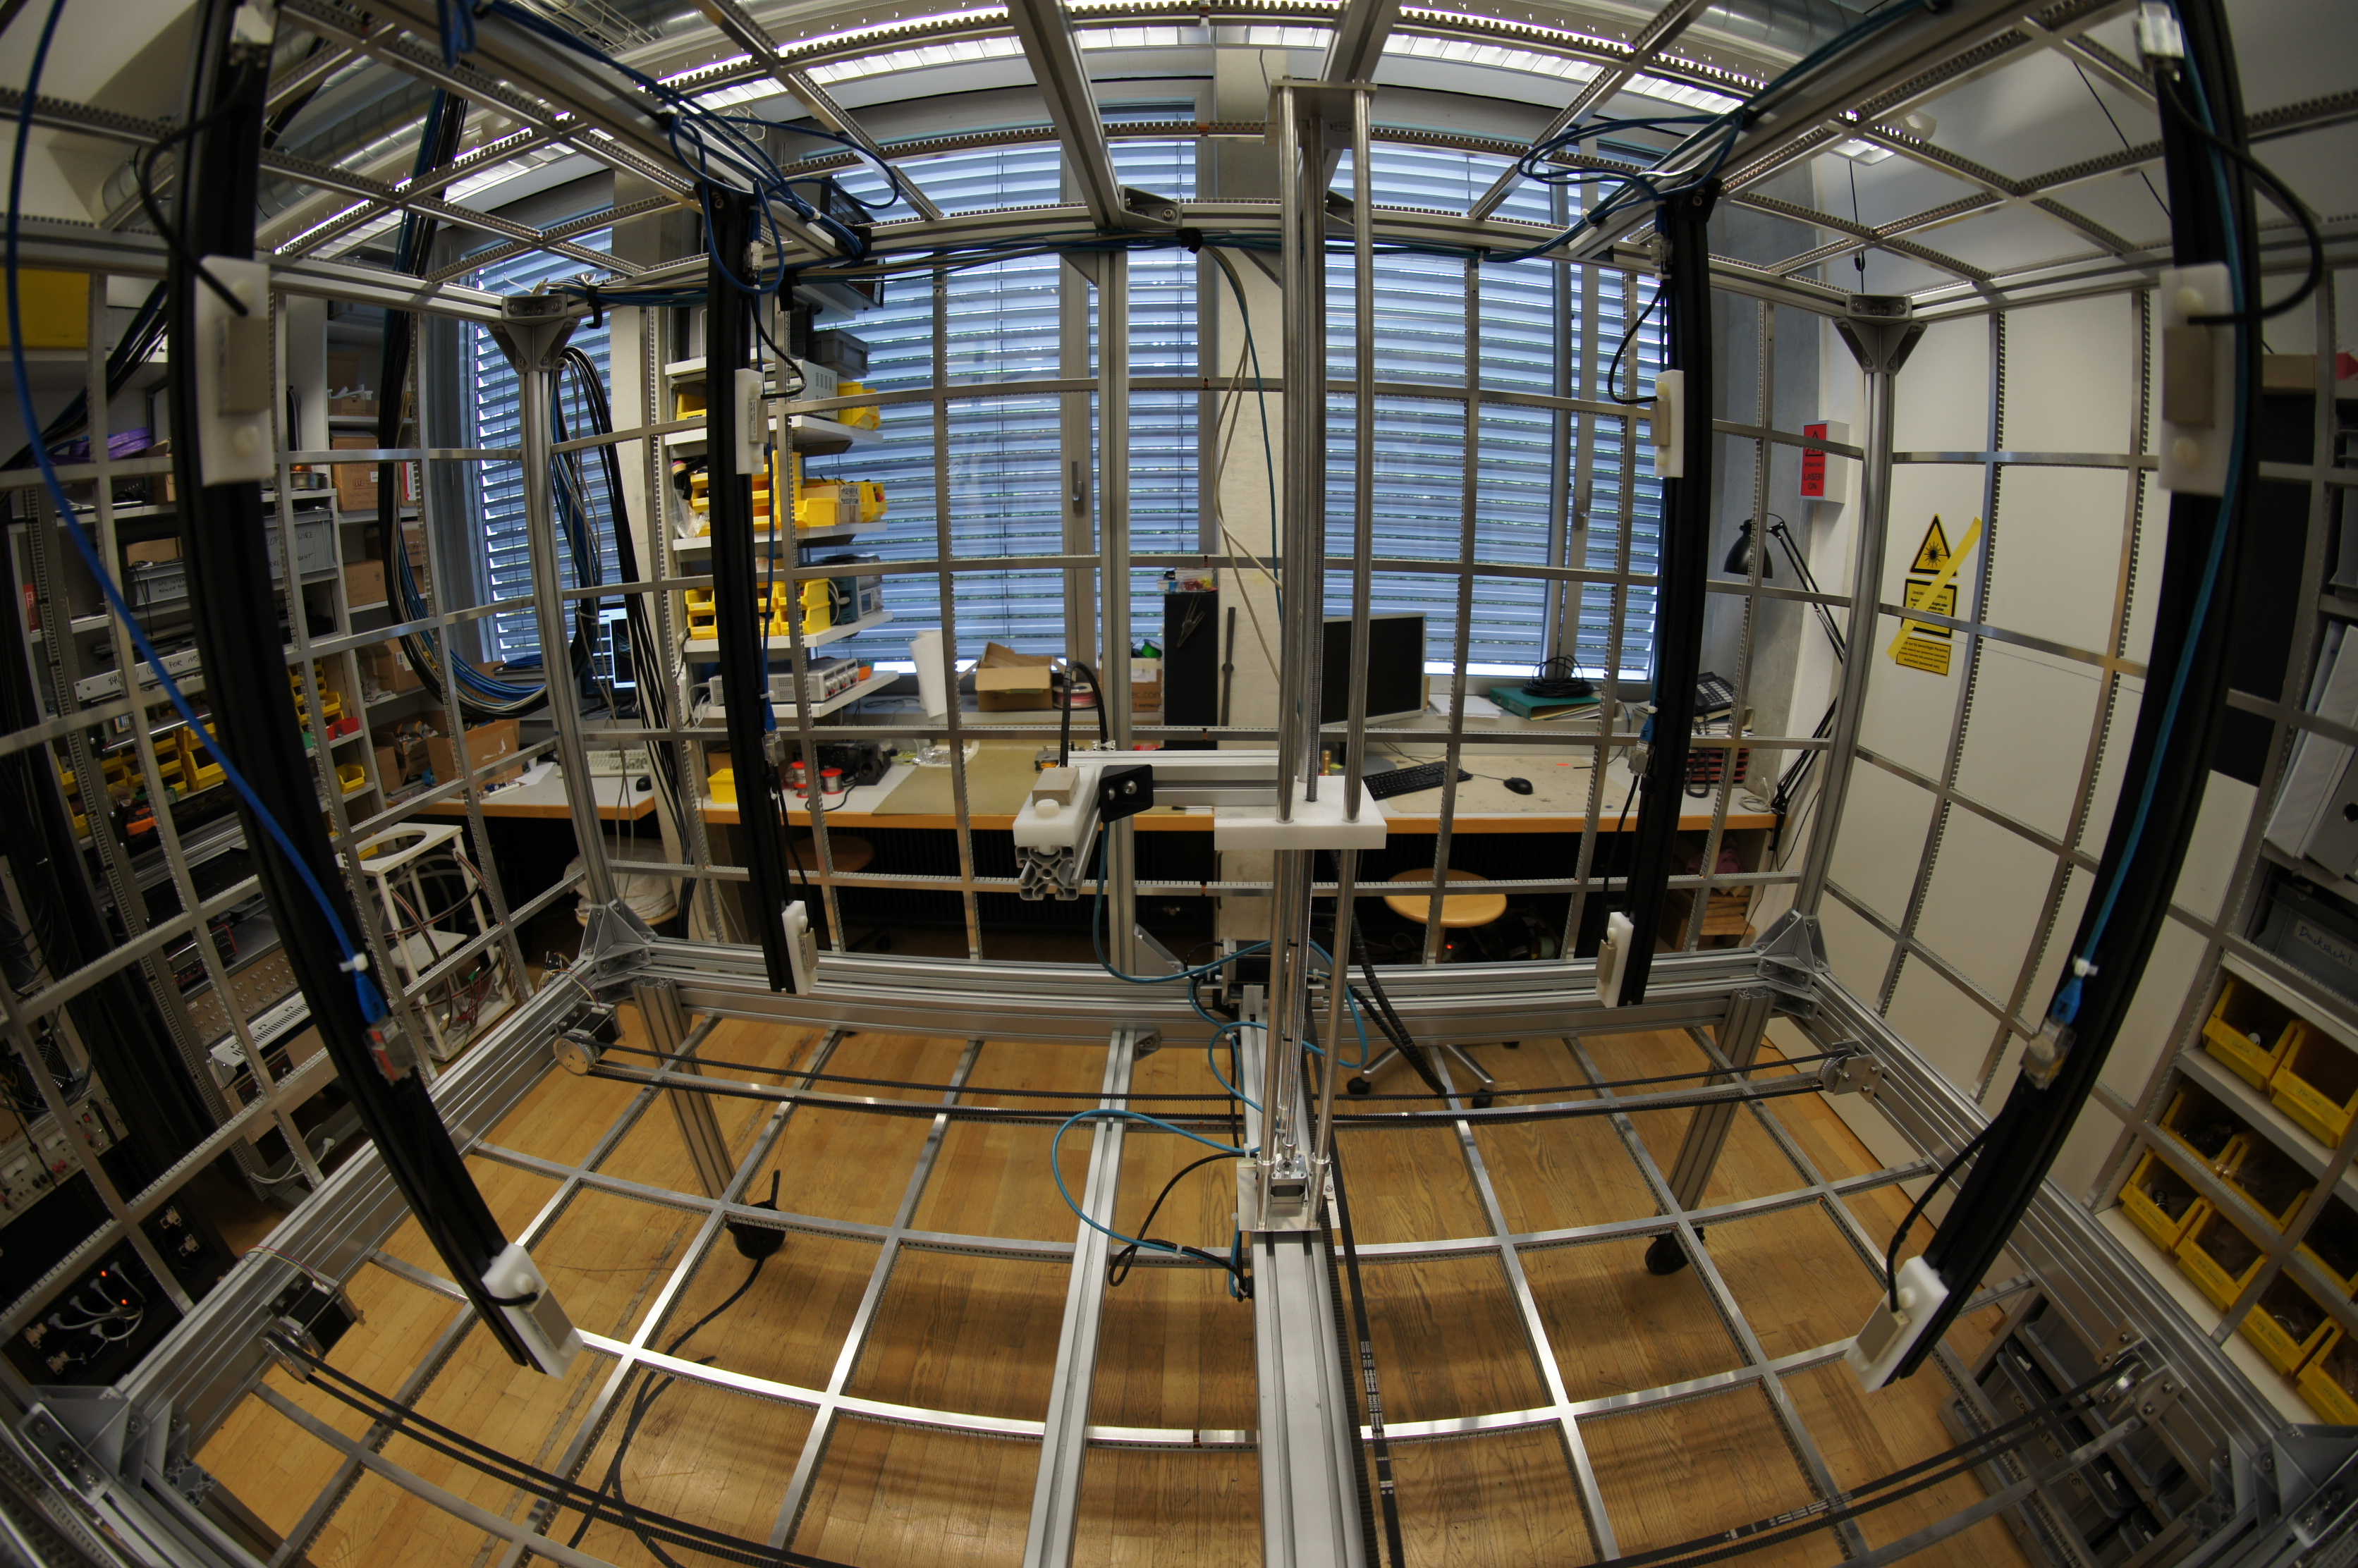
\includegraphics[width=0.9\linewidth]{gfx/prototype/DSC03476.JPG}
  \caption{The inside of the active magnetic field compensation system. In the centre the mapping robot (\emph{mapper}) is visible, with a fluxgate magnetic field sensor mounted to a movable platform. Mounted on black, vertical beams there are eight fluxgates for the active feedback.}
  \label{fig:prototype_photo_inside}
\end{figure}

A beam seen in the middle of Fig.\,\ref{fig:prototype_photo_inside} could move along the $y$ direction, pulled by two timing belts. The belts were wound around pulleys attached to stepper motors, visible to the left. Along the beam, the $x$ direction, a cart was moved in the same way---a timing belt and a stepper motor. On the cart three vertical rods were attached, with a plastic (POM) platform tightly threaded on them. On the platform there was a fluxgate magnetic field sensor. In the middle of the rods there was an aluminum threaded rod, passing through a threaded hole in the platform and mounted to a stepper motor on the cart. As the motor spun the threaded rod, the platform moved vertically, along the $z$ direction.

A simple kind of map possible with the mapper is a linear one, whereby the fluxgate was moved along one direction only. A map of the $y$-coil, mapped along the $y$ direction (in the middle of $x$ and $z$), is shown on the right-hand side in Fig.\,\ref{fig:prototype_linear_map} (only the $y$-component of the magnetic field is plotted, the coil was set to produce \SI{50}{\micro\tesla}). The background field was also mapped and the plotted map has it already subtracted. The field stayed in a \SI{\pm 0.2}{\micro\tesla} range around the average value.

\begin{figure}
  \centering
  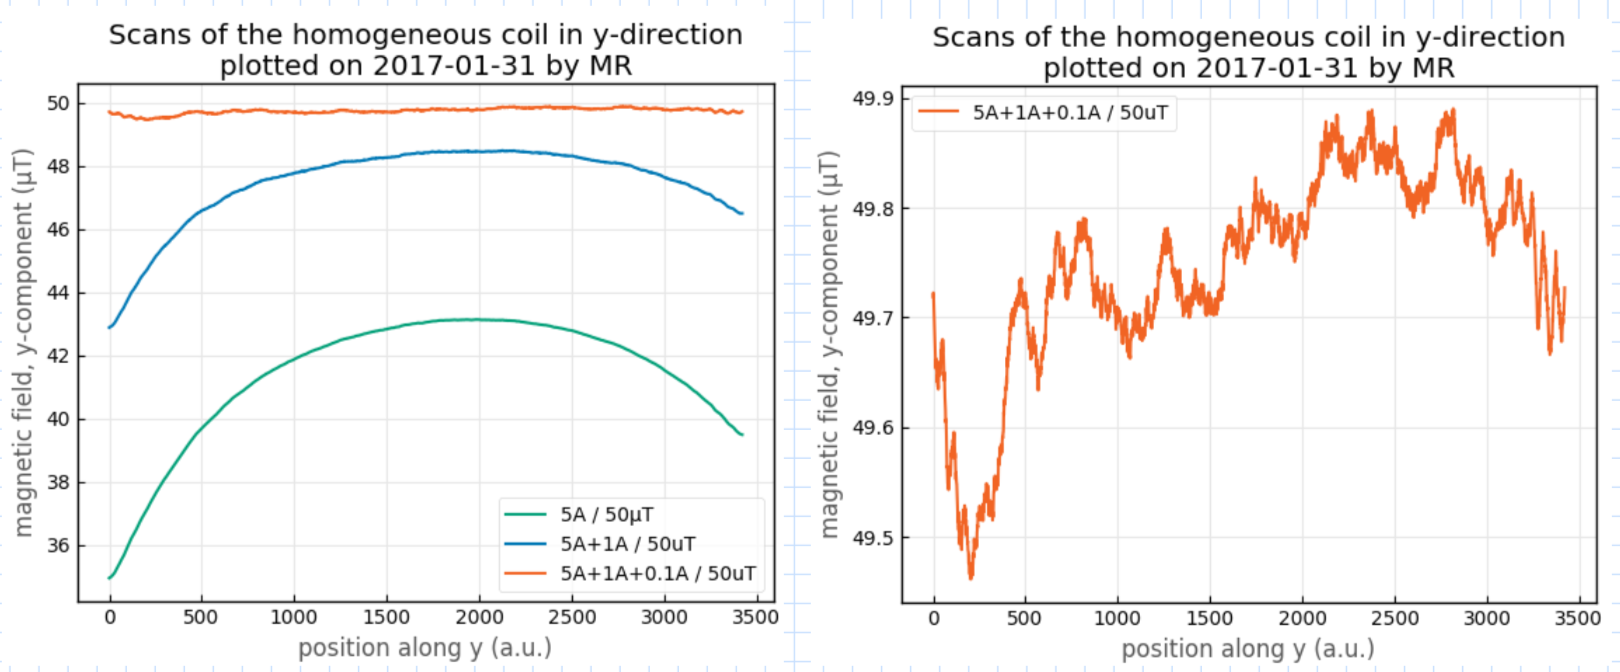
\includegraphics[width=0.9\linewidth]{gfx/prototype/linear_map.png}
  \caption{Right-hand side: Linear map of the homogeneous field $y$-coil. The map is along the $y$-direction, in the middle of $x$ and $z$. The $y$-component of the magnetic field is plotted. On the left-hand side additionally maps with only the \SI{5}{\ampere} component coil, and with \SI{5}{\ampere} and \SI{1}{\ampere} components coil are shown.}
  \label{fig:prototype_linear_map}
\end{figure}

On the left-hand of Fig.\,\ref{fig:prototype_linear_map} additionally the maps with only the \SI{5}{\ampere} component coil, and with \SI{5}{\ampere} and \SI{1}{\ampere} components coil are shown. It is interesting to note how much of the field is produced by each of the components. In the middle region the \SI{5}{\ampere}, \SI{1}{\ampere} and \SI{0.1}{\ampere} components produced 86\%, 11\% and 3\% of the field, respectively. At the edge the shares change to 70\%, 16\% and 14\%. \note{These numbers give also the relative requirements for the components. Five times less stable? Makes no sense\ldots What would the requirements really be? Linearity, for example! Could use worse power supplies.}

Another type of map is a planar one. A horizontal map, in the middle $xy$-plane, of the $y$-coil is presented in Fig.\,\ref{fig:prototype_plane_map}. The plot shows the maximum deviation among all three components of the magnetic field, i.e.\ in the area enclosed by the \SI{1}{\micro\tesla}~isocountour all components of the field are within \SI{1}{\micro\tesla} from the nominal field. The border of the plot corresponds to planes where the wires of the coils are. The fiducial volume is marked with grey lines. The field inside the fiducial volume stays within \SI{1}{\micro\tesla} of the nominal one of \SI{50}{\micro\tesla}, so the relative homogeneity is 2\%.
\mnote{Need to be clear about the specification---it wasn't supposed to be 2\% EVERYWHERE! Maybe bring forward the specification plot that decided on the grid size?}

\begin{figure}
  \centering
  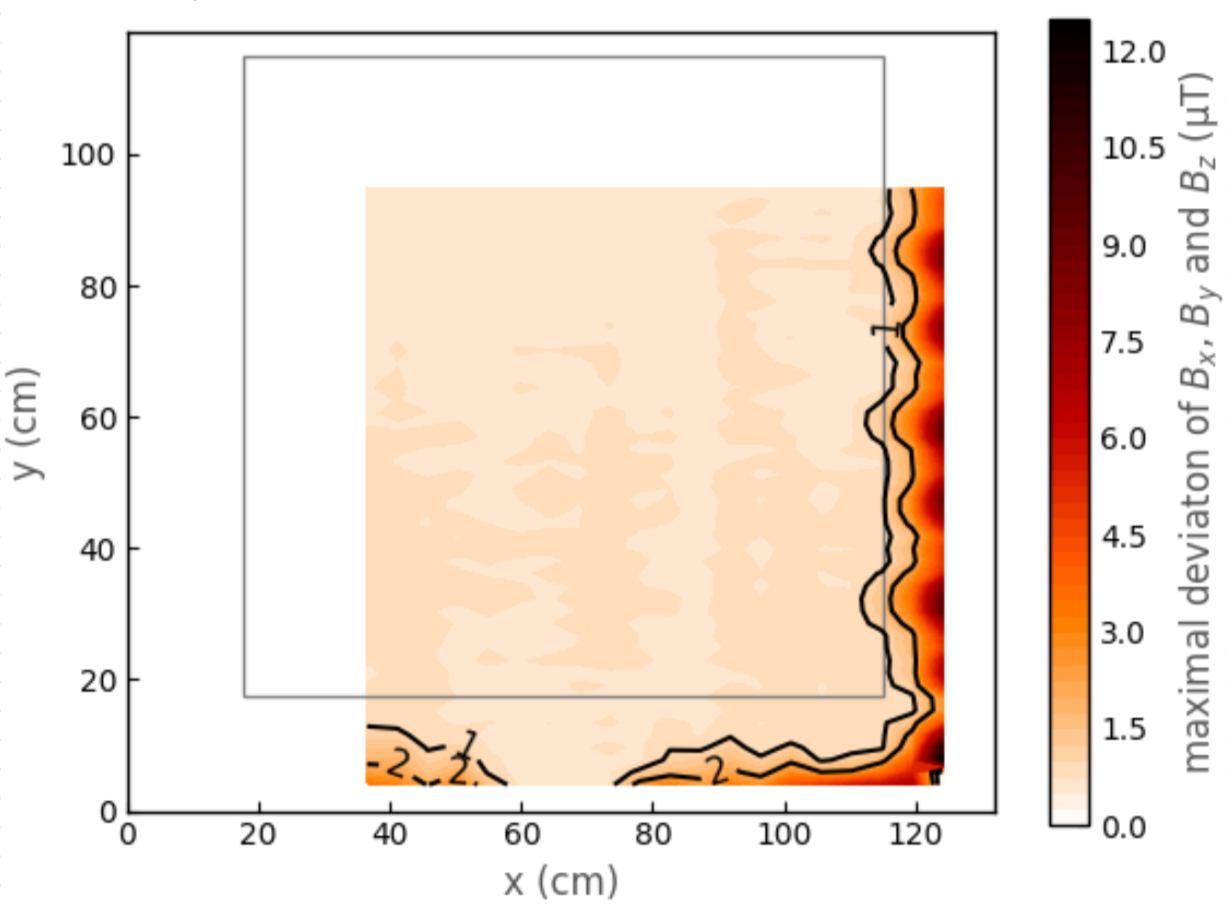
\includegraphics[width=0.9\linewidth]{gfx/prototype/plane_map.png}
  \caption{A horizontal map, in the middle $xy$-plane, of the $y$-coil. The maximum deviation among all three components of the magnetic field is plotted, i.e.\ in the area enclosed by the \SI{1}{\micro\tesla}~isocountour all components of the field are within \SI{1}{\micro\tesla} from the nominal field. The border of the plot corresponds to planes where the wires of the coils are. The fiducial volume is marked with grey lines.}
  \label{fig:prototype_plane_map}
\end{figure}



\section{DAQ}
Before proceeding to discuss the active stabilisation system, we devote a section to the hardware. These are technical details, but for the more tech-savvy of the readers haveing the hardware setting given first may ease following the discussion.

Already in Sec. \note{ref to the beginning} we set the frame of the active magnetic field stabilisation system. A change in the magnetic field is detected with an array of sensors, an appropriate response is calculated and applied by driving a change in currents flowing in the coils. The feedback loop is closed through the air when the sensors detect the change in the field caused by the coils.

\marginpar{In a fluxgate a ferromagnetic core is periodically driven into saturation. When it is not saturated, it is highly permeable and sucks the external magnetic flux in. When saturated, it does not occur. A pickup coil detects the changes in the external flux as it is alternately sucked in and out of the core.}

The field was measured with eight fluxgates, visible in Fig.\,\ref{fig:prototype_photo_inside}.
The sensors were Stefan Mayer Instruments FLC3-70 three-axis fluxgates, \SI{\pm 200}{\micro\tesla} range, \SI{1}{\kilo\hertz} bandwidth, $\pm 1\% \pm \SI{0.5}{\micro\tesla}$.
They were powered with an in-house--built double \SI{\pm 5}{\volt} power supply. The outputs of the fluxgates were \SI{\pm 5}{\volt} signals proportional to the magnetic field.
The analogue signals were directly digitised with 16-bit Beckhoff EL3602 24-bit differential analogue-to-digital converters (ADCs). The digital information was collected in software running on a PC computer.

The software stack, running under OpenSUSE Linux, consisted of a low-level Ethercat driver~\cite{etherlabcode} on top of which a custom program, written in \texttt{julia}~\cite{julia}, was running. This setup was optimised for high flexibility and close-to-zero turnaround time. In particular, it was possible to develop the software interactively \emph{while} the system was running. Besides the usual recording and graphically plotting the data, the main task of the software was to evaluate the optimal response for the measured magnetic field changes. The optimal response, the new currents to be applied to the coils, was sent to the digital-to-analogue converters (DACs).

\marginpar{The main julia program published the data on a \texttt{ZMQ} \texttt{PUB} socket. The data were stored with a separate \texttt{julia} program, collecting the data on a \texttt{ZMQ} \texttt{SUB} socket. Similarily, the plotting program was separate, written in \texttt{Python}.}

The DACs were 16-bit Beckhoff EL4134. The signals were then amplified with an array of four-quadrant SERVOWATT amplifiers, configured to amplify the voltage input to a current output. \note{Put here the exact amplifiers}. The currents were then directly fed into the coils.

\begin{SCfigure}
  \centering
  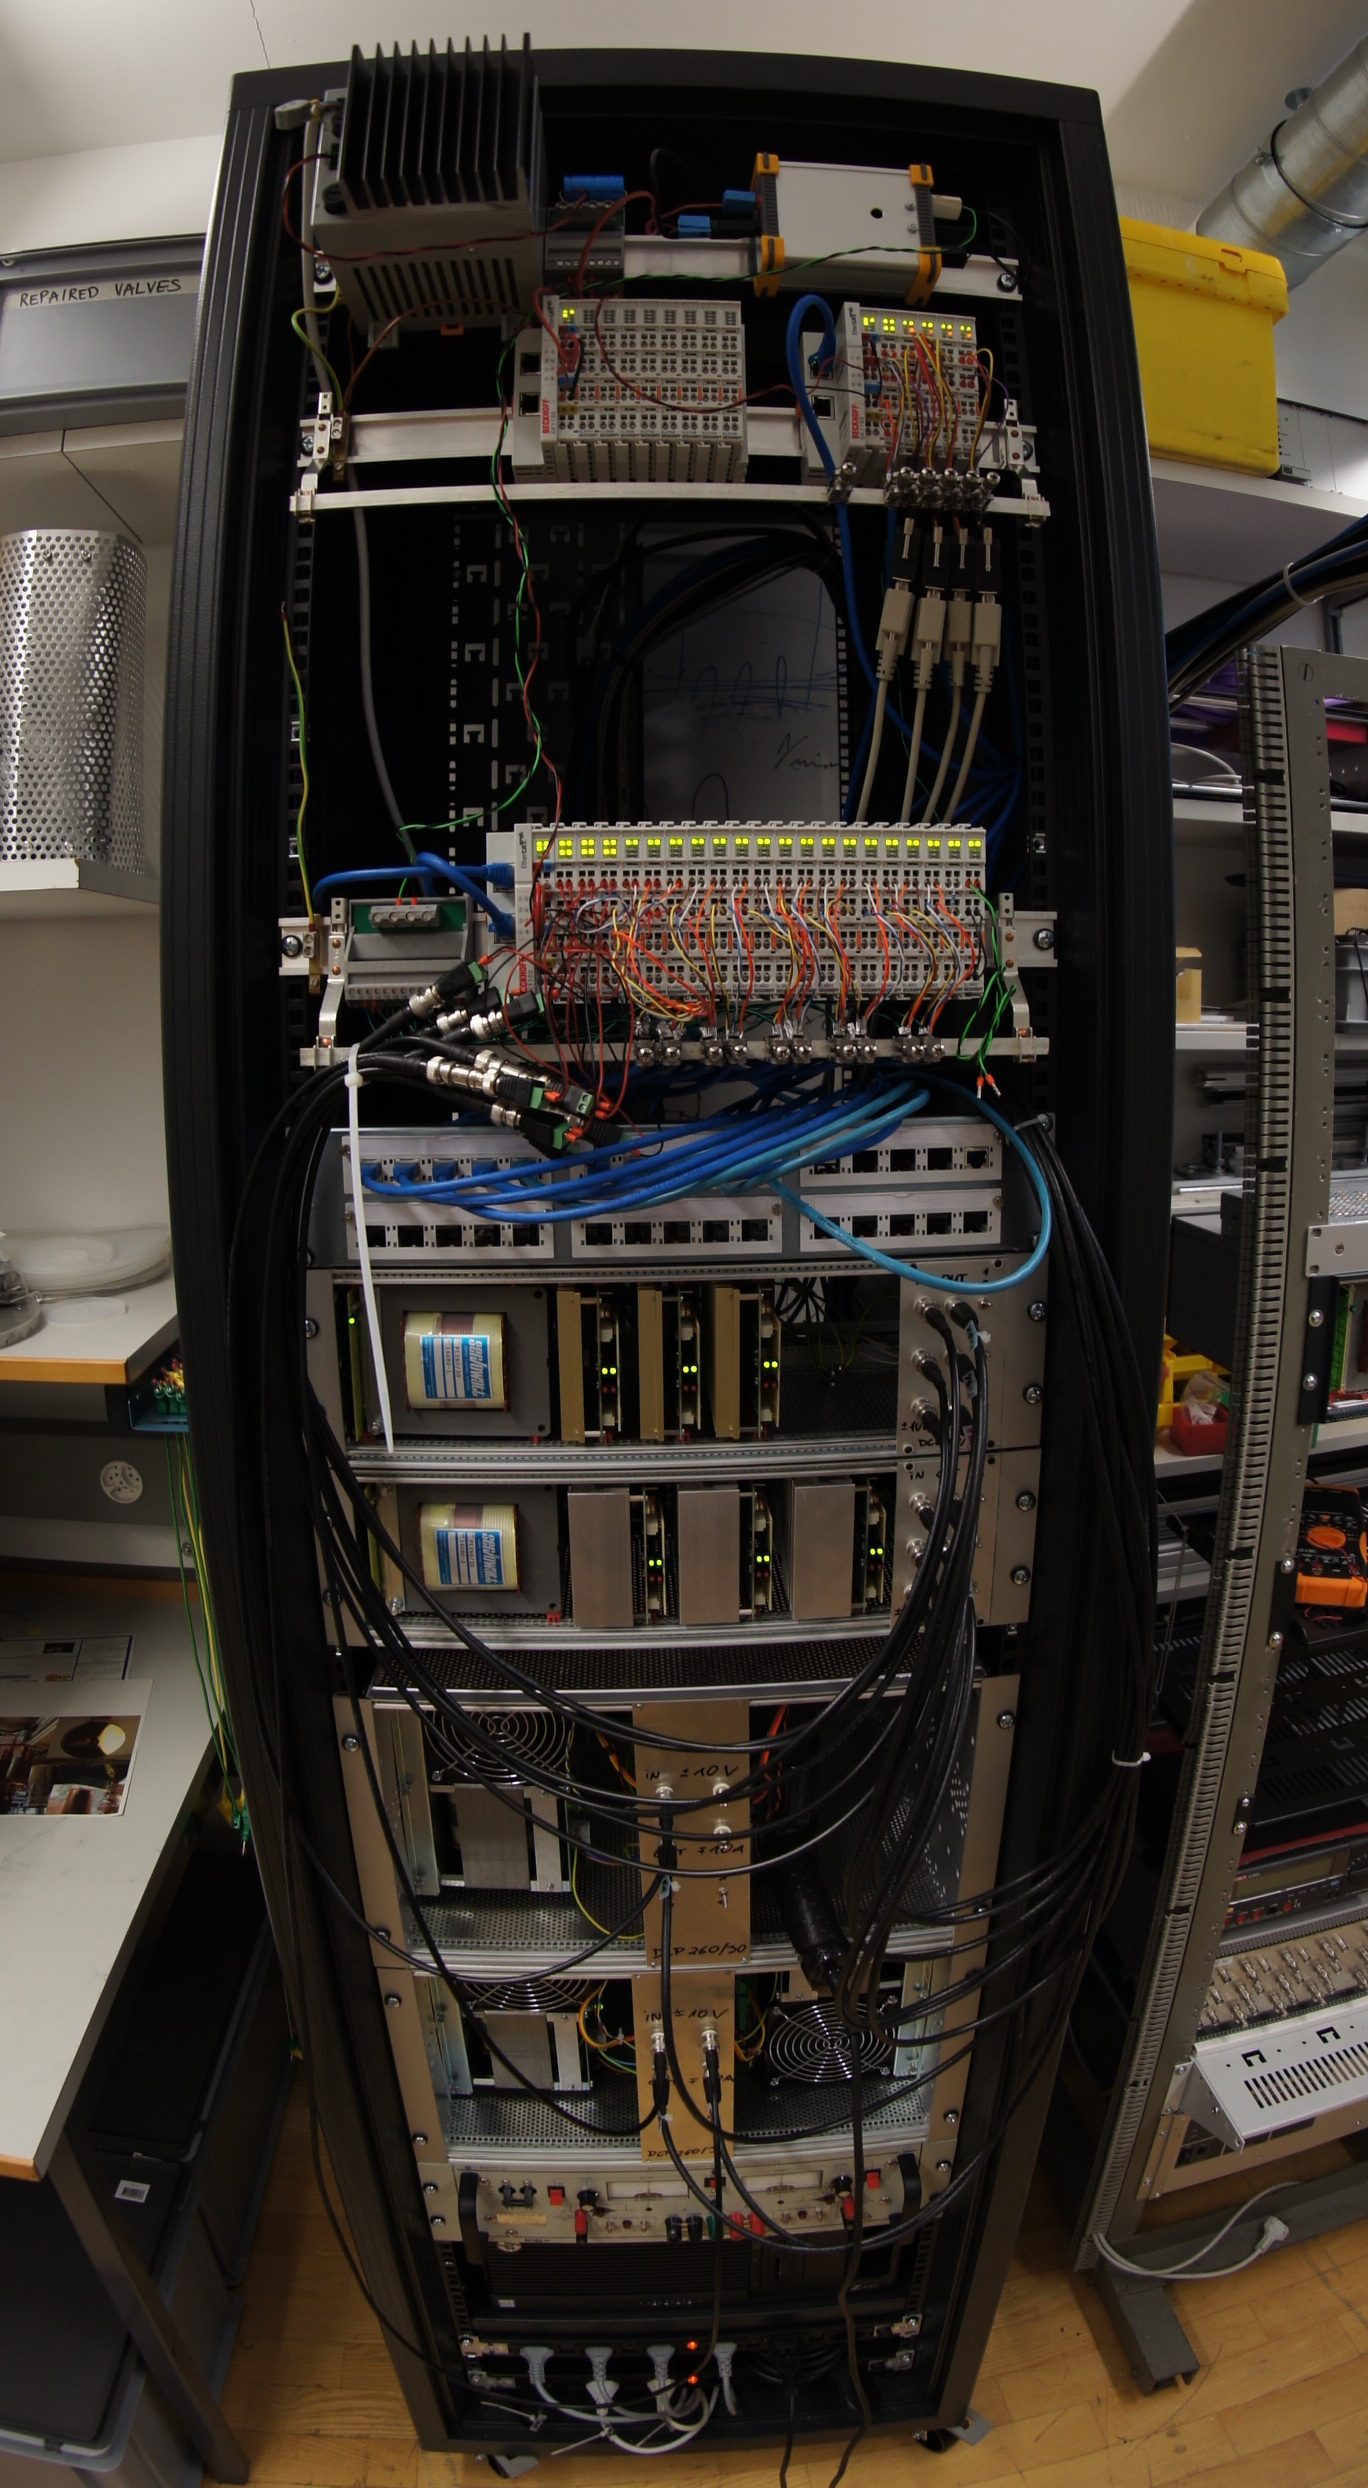
\includegraphics[width=0.4\linewidth]{gfx/prototype/DSC03477_cropped.jpeg}
  \caption{The 19-inch cabinet hosting the electronics for the active magnetic field stabilisation system. From top: a \SI{24}{V} power supply for the Beckhoff EtherCAT clamps and in-house--built \SI{\pm 5}{\volt} power supply for the fluxgates; spare EtherCAT clamps and control system for the mapper; a large array of EtherCAT DACs and ADCs for the active stabilisation system; breakout panel for the fluxgate cables (RJ-45 plugs); subrack with \SI{\pm 0.2}{A} amplifiers; subrack with \SI{\pm 2}{A} amplifiers; two subracks with \SI{\pm 10}{A} amplifiers; a general-purpose Kepco \SI{\pm 20}{V} \SI{\pm 20}{A} four-quadrant amplifier; the PC.}
  \label{fig:prototype_photo_daq}
\end{SCfigure}

The hardware was hosted in a 19-inch cabinet, pictured in Fig.\,\ref{fig:prototype_photo_daq}. A detailed list of the components can be found in the Figure's caption. This is all that, additionally to the coils themselves, was used to set up the active magnetic field compensation.


\section{The SFC matrix}
The system, fluxgates and coils, is fundamentally linear. The magnetic field seen by each of the 24 sensors is linear with the currents in the three coils, not unlike the discussion in Sec.\,\ref{ch:coil_design}. All readouts, gathered in a vector $\mathbb{B}$ (dimension 24) can be written as a linear combination of the currents in the coils $\mathbb{I}$ (dimension 3):
\begin{equation}
  \label{eq:SFC_matrix_model}
  \mathbb{B} = M \mathbb{I} + \mathbb{B}_0 \ .
\end{equation}
\marginpar{We use the letter $\mathbb{B}$ for the values measured by the sensors to distinguish it from $\bm{B}$, which is used to denote the magnetic field in the whole space.}
$\mathbb{B}_0$ is the free offset. The matrix of proportionality constants $M$, dimension $24 \times 3$ \note{verify}, is the central element of the active magnetic field compensation. It is called the response matrix or the SFC matrix \note{need to establish the nomenclature}. 
\note{Need to see how much I explain in the nEDM SFC at the beginning.}

The SFC matrix of the nEDM@PSI SFC system and its properties were thoroughly discussed in Sec.\,\ref{fig:nEDM_SFC_matrix}. There is a fundamental difference between the matrix of the nEDM@PSI system and the next generation one. The nEDM@PSI's matrix was not known a priori. The system was constructed and the matrix was measured as the system's property.
This could be considered as the reason that the matrix was ill-conditioned and the system required regularisation and PI control to be stable.
Conversely, the new system takes the matrix into account already at the design phase. The coils are designed to produce magnetic field corresponding to the terms of the Cartesian harmonic expansion of the field.
\note{Needs to be clear here!} This ensures that they are orthogonal to one another. We expect the matrix to have the condition number equal to 1.

\note{Put a figure about the measurement of the matrix?}

The active magnetic field compensation system constructed at ETH implemented a new way of measuring the matrix. Not only it changes currents in all the coils simultaneously, shortening the duration of the procedure, but can also measure in close-to-zero field conditions.

To measure the matrix we considered the space spanned by all the coils. In this case it was three-dimensional---the current in the $x$-coil, in the $y$-coil and in the $z$ one. A point in this space corresponds to one configuration of the currents in the coils. We picked a set of points on an n-sphere in this space and continuously changed the currents to walk from one point to another. As all the currents were simultaneously changed, the measurements of the sensors were recorded. Then for each readout channel ($8 \times 3 = 24$ in total) a linear model was fitted to estimate the proportionality constants between the readout and the currents in the coils:
\begin{equation}
  \label{eq:SFC_matrix_linear_fits}
  B_i = B_i^0 + \sum_{j=x,y,z} M_{i,j} \, I_j \ ,
\end{equation}
where $B_i$ is the readout channel ($i$ going from 1 to 24), $I_j$ are the currents in the coils ($j$ going over $x$, $y$ and $z$) and $M_{i,j}$ is the matrix of proportionality constants---the SFC matrix. $B_i^0$ is the free offset vector---the background field.
\note{Sort out the indexes, which is which.}

If the system is perfectly linear it does not matter where in the current-space the n-sphere is located, nor how large it is (though larger give more precise estimates per point). We expect, however, nonlinearities to appear in the presence of a mu-metal shield.
In that case it is preferable to measure the matrix in the vicinity of the point where the system is later operated. Following this motivation the following procedure of the matrix measurement was employed: First an n-sphere centred at n-zero and a radius of \SI{50}{\micro\tesla} was chosen. Then the system walked over ten random points on the sphere, taking two seconds to go from one to the next (\SI{20}{\second} in total).
\marginpar{It is possible to fit the linear model and estimate the uncertainty of the matrix elements \emph{while} measuring; the measurement can be stopped when the uncertainty drops below a threshold.}
This gave the first estimate of the matrix. The next sphere is chosen to be centred around the zero field. This is the optimal, in the least-squares sense, solution of Eq.\,\ref{eq:SFC_matrix_model} with $\mathbb{B} = 0$ (exactly as it was the case in Eq.\,\ref{eq:requirement}):
\begin{equation}
  \label{eq:SFC_zero_field_requirement}
  \mathbb{I}_\text{zero-field} = M^\dagger \, \mathbb{B}_0 \ ,
\end{equation}
where $\mathbb{B}_0$ is the free offset from Eq.\,\ref{eq:SFC_matrix_linear_fits} and $M^\dagger$ is the Moore-Penrose pseudoinverse of the matrix $M$. This gave the second estimate of the matrix. Finally, the measurement was repeated with a sphere again centred at zero, but with a smaller radius of \SI{0.1}{\micro\tesla}. The procedure was developed for a system with mu-metal. \note{but is beautiful in any way} In the case of an air system all consecutive estimates of the matrix were the same.

A typical measured matrix is\ldots Estimate the field inhomogeneity right away from it! Give two at two distances, maybe?

Then continue to analyse the matrix. Discuss the SVD decomposition and its singular values. Or is it the right place to do it here?


\section{The feedback algorithm}
The feedback is based on calculating the optimal solution of the Eq.\,\ref{eq:SFC_matrix_model} in each step. This is in contrast to stabilisation and control approach taken in the previous system.

We start at the $n$th iteration (the iteration index marked on top) with Eq.\,\ref{eq:SFC_matrix_model}:
\begin{equation}
  \mathbb{B}^n = \mathbb{M} \mathbb{I}^n + \mathbb{B}_0^n
\end{equation}
For the next iteration we want the field to be equal to the target field (which we allow to be any): $\mathbb{B}^{n+1} \overset{!}{=} \mathbb{B}_\text{target}$, which is leads to the following requirement for the next currents:
\begin{align}
  \mathbb{I}^{n+1} &=
    \mathbb{M}^\dagger \left( \mathbb{B}_\text{target} - \mathbb{B}_0^{n+1} \right) \nonumber \\
    &\approx \mathbb{M}^\dagger \left( \mathbb{B}_\text{target} - \mathbb{B}_0^{n} \right) \nonumber \\
    &= \mathbb{M}^\dagger \left( \mathbb{B}_\text{target} - \mathbb{B}^n + \mathbb{M} \mathbb{I}^n \right) \nonumber \\
    &= \mathbb{M}^\dagger \left( \mathbb{B}_\text{target} - \mathbb{B}^n \right) + \mathbb{M}^\dagger \mathbb{M} \mathbb{I}^n \nonumber \\
    &= \mathbb{M}^\dagger \left( \mathbb{B}_\text{target} - \mathbb{B}^n \right) + \mathbb{I}^n \ . \label{eq:current_update}
\end{align}
By defining $\Delta\mathbb{I}^n := \mathbb{I}^{n+1} - \mathbb{I}^{n}$ and $\Delta\mathbb{B}^n = \mathbb{B}^n - \mathbb{B}_\text{target}$ we obtain the intuitive rule for the current update:
\begin{equation}
  \Delta\mathbb{I}^n = - \mathbb{M}^\dagger \Delta\mathbb{B}^n
\end{equation}
A careful reader may be alarmed by the approximation $\mathbb{B}_0^{n+1} \approx \mathbb{B}_0^{n}$. It is true that it does not hold in practice, but is nevertheless an unfortunate necessity. For the calculation needs to be performed just before the iteration $n+1$, when $\mathbb{B}_0^{n+1}$ is not yet known. In other words, the correction is delayed by one iteration. This introduces a lag in the system and motivates high feedback frequencies.

In practice the system had a delay of more than one iteration. Although the system was operated at \SI{200}{\hertz} the quickest turnaround was three cycles. This was tested by applying a pulse on an DAC channel and observing the response on a directly connected ADC channel. Knowing that the magnetic field information is delayed, it was crucial to delay the current information, too, so that Eq.\,\ref{eq:current_update} became:
\begin{equation}
  \mathbb{I}^{n+1} = \mathbb{M}^\dagger \left( \mathbb{B}_\text{target} - \mathbb{B}^{n-2} \right) + \mathbb{I}^{n-2} \ .
\end{equation}
Without accounting for the delay the system would spontaneously destabilise.

\note{Put the step-response plot? Depending how crowded with plots it is later.}

\note{A paragraph (or a margin note) comparing the feedback algorithm to the old one. Requires no parameters, any field may be the target field.}

\note{Has been tested with the big system, but it did not outperform in terms of stability (do I have a plot to prove that?). Nick Schwegler's project report! I could just cite it here, it was inconclusive. But for sure I can say it.}




\section{Dynamic stabilisation}
The dynamic stabilisation was tested with a strong permanent magnetic dipole. It was build out of two extremely strong neodymium magnets (\SI{200}{\kilo\gram} force when attached to iron) connected with an iron rod. The dipole was moved by hand several meters from the system causing magnetic field disturbance.

\mnote{Need to put the details of the geometry of the fluxgates here. Eight fluxgates on the corners of a cube of \ldots size.}

\begin{figure}
  \centering
  \subfloat{
    \label{fig:prototype_compensation_time_1}
    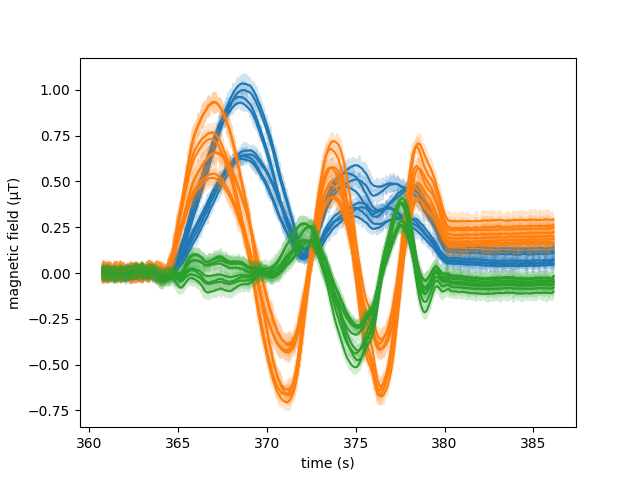
\includegraphics[width=.45\linewidth]{gfx/prototype/uncompensated_7_5m.png}}
  \quad
  \subfloat{
    \label{fig:prototype_compensation_time_2}
    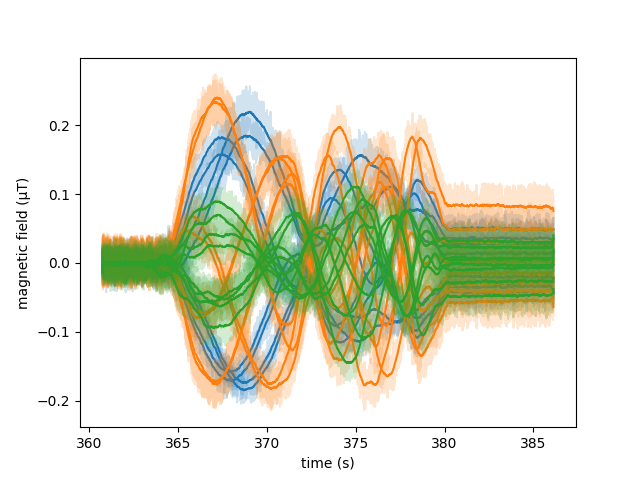
\includegraphics[width=.45\linewidth]{gfx/prototype/compensated_7_5m.png}}
  \caption{Field variations caused by a dipole \SI{7.5}{\meter} away being rotated. Left-hand side: uncompensated field $\mathbb{B}_0$ (as calculated with Eq.\,\ref{eq:uncompensated_field}). Right-hand side: compensated field seen by the feedback sensors $\mathbb{B}$. The three colours correspond to the three spatial directions. Each line is one feedback sensor. The thick lines are downsampled data, the original being plotted in light colour below.}
  \label{fig:prototype_compensation_time}
\end{figure}

The result of the compensation of the dipole being rotated \SI{7.5}{\meter} away from the system's centre are plotted in Fig.\,\ref{fig:prototype_compensation_time}. The left-hand--side plot shows the field as it would be registered without compensation $\mathbb{B}_0$ calculated according to Eq.\,\ref{eq:SFC_matrix_model}):
\begin{equation}
  \label{eq:uncompensated_field}
  \mathbb{B}_0 = \mathbb{B} - \mathbb{M} \mathbb{I} \ .
\end{equation}
The three colours correspond to the three spatial components ($x$, $y$, $z$). Each line is one sensor. On the right-hand side the actually measured field $\mathbb{B}$ is depicted. We see that the amplitude of the changes was reduced from around \SI{1.75}{\micro\tesla} to \SI{0.4}{\micro\tesla} (factor four). Yet, the variation is not mitigated completely and the reason in quite fundamental.

Take a look on the orange lines on left-hand side of Fig.\,\ref{fig:prototype_compensation_time}, each representing the readout of a different sensor in the $y$ direction. They do not overlap, which means that the field change was not homogeneous (which, of course, would be the same everywhere). The coils of the system, being able to generate only homogeneous fields, can only compensate the homogeneous part. Graphically it may be explained in the following way: each of the coils coil can keep all lines in one of the colours (one spatial component) steady, but it cannot bring them closer together (homogenise the field). This is what can be observed on the right-hand side of Fig.\,\ref{fig:prototype_compensation_time}. There lines are centred around zero, but their spread within one colour (spatial component) is not reduced. After all, the active compensation can compensate only as much as it can.

\begin{figure}
  \centering
  \subfloat{
    \label{fig:prototype_compensation_performance}
    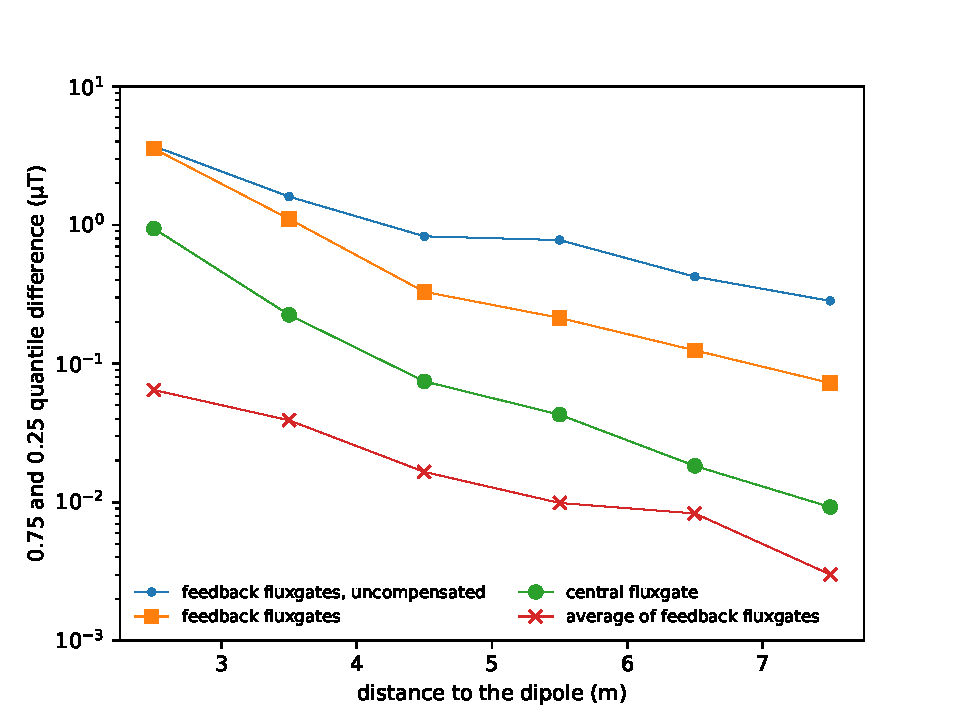
\includegraphics[width=.45\linewidth]{gfx/prototype/big_magnet_performance.pdf}}
  \quad
  \subfloat{
    \label{fig:prototype_shielding_factor}
    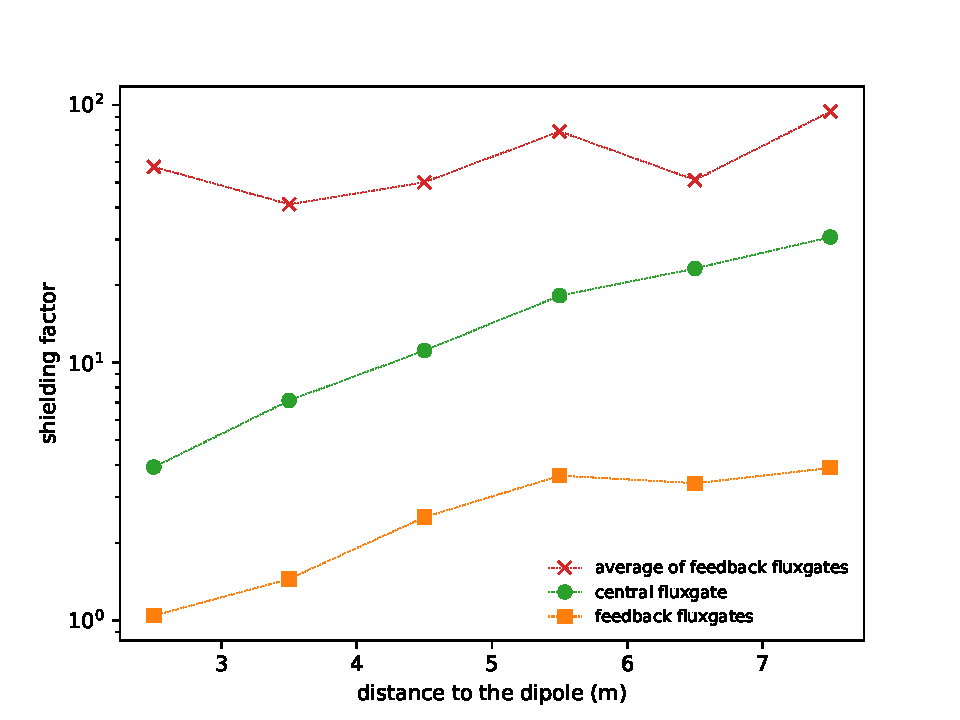
\includegraphics[width=.45\linewidth]{gfx/prototype/big_magnet_shielding_factor.pdf}}
  \caption{Performance of the active compensation system shielding a dipole disturbance, as a function of the distance to it. Left-hand side: the amplitude of the field variations, measured as the difference between the 75th and 25th quantiles, as uncompensated (blue), compensated seen by the feedback sensors (orange), a non-feedback sensor in the centre (green) and the numerical average of the feedback sensors (red). Right-hand side: the shielding factor, defined as the ratio of the curves in the plot to the left to the uncompensated variation.}
  \label{fig:prototype_compensation}
\end{figure}

The amplitude of the variations seen in Fig.\,\ref{fig:prototype_compensation_time} can be quantified as the difference between 75th and 25th quantiles of the readouts. This measure is plotted in the left-hand side of Fig.\,\ref{fig:prototype_compensation} as the function of the distance between the dipole disturbance and the centre of the system. The uppermost curve, blue, is the uncompensated field $\mathbb{B}_0$, the left-hand side of Fig.\,\ref{fig:prototype_compensation_time}. The orange one below is the compensated field seen by the feedback sensors $\mathbb{B}$, the right-hand side of Fig.\,\ref{fig:prototype_compensation_time}. We observe that the compensation improved with the distance to the dipole, as the field became more homogeneous. It is more clear in the right-hand side, where the ratio of the two curves, called the \emph{shielding factor}, is plotted in orange.

The next curve, green, corresponds to the field measured by a sensor placed in the middle of the system. There the system compensates 1st-order changes (because they are anti-symmetric with respect to the centre). It suggests that the difference to the shielding factor for the feedback sensors, a factor three, can be attributed to the uncompensated variations of 1st-order gradients. Furthermore, it suggests that if the system would be extended by a addition of 1st-order coils the shielding factor for the feedback sensors (in the whole volume) would be as good as for the centre.

The last, red, curve depicts the variations seen in the average readout of the feedback fluxgates. A perfect system should compensate it perfectly, regardless of the shape of the field changes. Yet the shielding factor for this measure was around 50. It also did not depend on the distance to the dipole (homogeneity of the field), suggesting that it is a property of the compensation system itself. The dominant factors are probably the finite reaction time and the inhomogeneity of the field created by the compensation coils. Even if the field changes, similar in magnitude and pace to the ones discussed, would be perfectly homogeneous, this system is not likely to compensate them better.


\section{Long-term Stability}
\marginpar{In the PSI environment periods of strong magnetic field changes---tens of microteslas over an hour when nearby magnets ramp---are interleaved with ones of high stability---\SI{10}{\nano\tesla} at \SI{10}{\second} at night (Fig.\,5.3 in \cite{Franke2013}).}
As we have just shown the active magnetic field compensation can stabilise the field in the case of strong variations. Yet, the system's internal stability is inevitably finite and when the magnetic environment is more stable, the system effectively worsens the conditions. The question is where is this limit and what sets it.

As the measure of stability we use the \emph{Allan deviation}---a special case of the M-sample variance, defined originally by the Eq.\,11 in~\cite{Allan1966}, with $N=2$ and $T = \tau$. The interpretation is: Allan deviation gives the RMS sample-to-sample variation \note{Write more on that, but not too much.}

To assess the stability the system run in the night, with no known activity in the immediate surrounding of the laboratory. The registered stability is plotted in Fig.\,\ref{fig:prototype_stability}. The colour convention follows the one of Fig.\,\ref{fig:prototype_compensation_time}---the three spatial components are depicted with blue, orange and yellow and each line corresponds to one sensor. The three uppermost groups of curves mark the stability of the uncompensated field $\mathbb{B}_0$ (as calculated with Eq.\,\ref{eq:uncompensated_field}). That the stability differs between the spatial components is not worrying---there is no reason to expect whatever caused the disturbance to be anisotropic. Below, at around \SI{20}{\nano\tesla} over a wide range of integration time, is large group of curves. Among them are ones of the compensated field $\mathbb{B}$. Even in the most quiet of the conditions in the laboratory the system improved the stability several times.

\begin{figure}
  \centering
  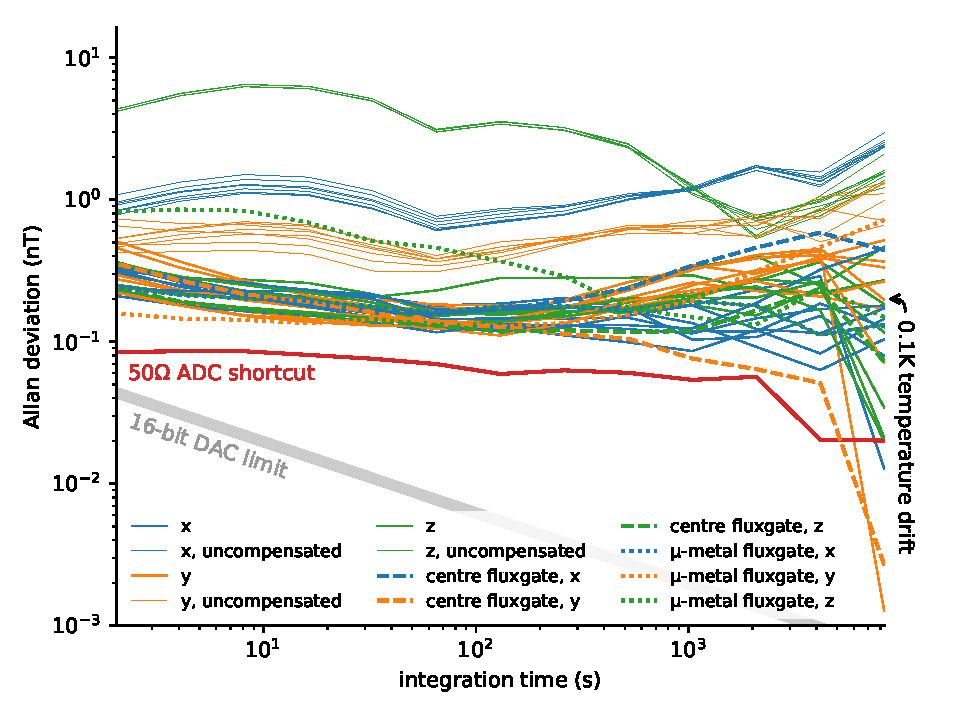
\includegraphics[width=0.9\linewidth]{gfx/prototype/run7_field_stability.pdf}
  \caption{The stability of the active magnetic field compensation. The Allan deviation is plotted as the function of integration time. The three colours depict the three spatial directions. The uppermost three groups of thin, solid lines depict the uncompensated field $\mathbb{B}_0$ measured by the feedback sensors. In the dense group of lines below, around \SI{20}{\nano\tesla} (corresponding to a temperature stability of \SI{0.1}{\kelvin}, as specified for the fluxgates), are: the compensated field measured by the feedback sensors $\mathbb{B}$ (solid), the compensated field measured by a non-feedback fluxgate in the centre of the system (dashed), field measured inside a two layer $\upmu$-metal shield (dotted). Below that depicted are: the stability of the readout of a short-cut ADC channel (red) and the limit set by the quantisation noise of the 16-bit DACs.}
  \label{fig:prototype_stability}
\end{figure}

In the previous section we already indicated that the field in the centre is stabilised better then the one at the feedback sensors in the case of high-order variations. In the plot the stability of the sensor in the centre is depicted with dashed lines. They lie in the large group around \SI{20}{\nano\tesla}, although rather on its lower side, suggesting that the variations during the measurement were homogeneous.

Why was not the improvement better? In the plot there seems to be a fixed limit for the stability. Another set of curves, the dotted ones, provide a hint. They depict the stability of the field observed with an additional sensor mounted inside a two-layer $\upmu$-metal shield, which should provide a factor of a hundred in shielding (the second layer was a cylinder without end caps aligned with the $z$-axis of the sensor, hence the worse performance in this direction). Yet, the registered stability is no better than that of the active stabilisation system.

The limit comes from the temperature drifts. According to the specification of the Stefan Mayer Instruments FLC3-70 sensor it drifts \SI{2}{\nano\tesla\per\kelvin}, so the observed stability corresponds to temperature stability as small as \SI{0.2}{\kelvin}. Even at night the temperature in a not air-conditioned laboratory cannot be expected to be more stable that that. This limit can be pushed a factor twenty lower with higher-quality (and higher-price) sensors. Commercially available Stefan Mayer Instruments FL1-100 and Bartington Mag-03 are specified to drift \SI{0.1}{\nano\tesla\per\kelvin} with a $\SI{\pm 100}{\micro\tesla}$ measuring range.

However, below is another limitation. Figure\,\ref{fig:prototype_stability} features also a red line labeled ,,\SI{50}{\ohm} ADC shortcut''. This is the stability of the readout of an ADC channel with the terminals connected with a \SI{50}{\ohm} resistor. Even if the magnetic field sensors would have output a perfectly stable voltage, the digitised information would be only this stable. A higher class digitisers could perform better.

The lowest curve on the plot is the limit on the stability due to the bit depth of the DACs. A quantisation resolution $\Delta$ corresponds, on average, to a white noise with RMS amplitude $\Delta / \sqrt{12}$ (derived for example in Sec.\,IV.A in \cite{Gray1998}). This noise scales then down as $\tau^{-1/2}$ with the integration time. The system's 16-bit DACs had $2^{16}$ levels mapped onto a $\SI{\pm 100}{\micro\tesla}$ range. This defines the quantisation at the feedback time of inverse $\SI{200}{\hertz}$. In total the limit from the quantisation at the integration time $\tau$ is:
\begin{equation}
  \frac{ \SI{200}{\micro\tesla} }{ 2^{16} \ \sqrt{12} \ \sqrt{ \SI{200}{\hertz}\ \tau} }
\end{equation}
Aside from the obvious---increasing the bit depth of the DACs---this limit can be pushed further by increasing the feedback frequency or decreasing the range of the operation.

Interestingly, the stability is fully defined by the measurement chain---the sensors and the digitisers. Instabilities of the output chain, DACs and amplifiers, indistinguishable from changes in the magnetic field, are corrected by the system itself.

\note{Maybe a paragraph comparing this stability to the PSI system}
% It should be noted that at PSI the stability registered was \ldots more stable than the ETH laboratory. Better sensors

\note{The process of winding a coil? Should be described!}


% \section{Testing the new feedback with the big system}
% Not sure where to put it, but somewhere in this chapter.

% Does not outperform, but is for example completely parameter-free (no I parameters), any field can be used as the target field.


\section{Open-design cage}
The disadvantage of the first-iteration design, pictured in Fig.\,\ref{fig:prototype_photo_inside} was that the cage is fully closed, making putting anything inside, or taking outside, quite a challenge. In particular, one of the areas the active magnetic field compensation system prototype could be used to investigate is the effects of a $\upmu$-metal shield inserted into it.

Three designs with the inside accessible were considered. In the first, connectors could be built in along edges of one of the faces (twenty, if the face is one of the small ones). To access the inside the connectors would have to be disconnected and then the face removed. The connectors would have to have as much as 30 pins, each connected to at least \SI{1}{\milli\meter} wire. 
\marginpar{D-subminiature connectors with soldering contact were considered for this purpose. Two per edge.} The process of winding a coil would be much to much.
Adding more coils would mean exchanging all connectors.

The second design featured a removable face without the need for connectors. The wires laid on one face would be separate from those on the rest of the structure. This would inevitably lead to some effective current cancellation along the edges of the removable face. \note{Explain why}.

The third way was to design a system with out wires on one face at all. This solution had the immediate advantage of demonstrating the power of the coil design method. The next iteration is designed with one face (rectangular one, $Y-$) left open. Designed fully following the algorithm.

A next improvement are 1st gradient coils. Even in the laboratory homogeneity\ldots bla, bla\ldots

The calculation with the fiducal volume of\ldots done for homogenous and 1st gradient coils. Fig.\,\ref{fig:prototype_open_design_simulation} presents the sections for... Fig.\,\ref{fig:prototype_open_design_Xcoil_coils} shows the first 22 (out of 64) current loops. \note{All with 1A wires? not much more} The numbers show the number of windings in the 5A, 1A and 0.1A scheme.

\begin{figure}
  \centering
  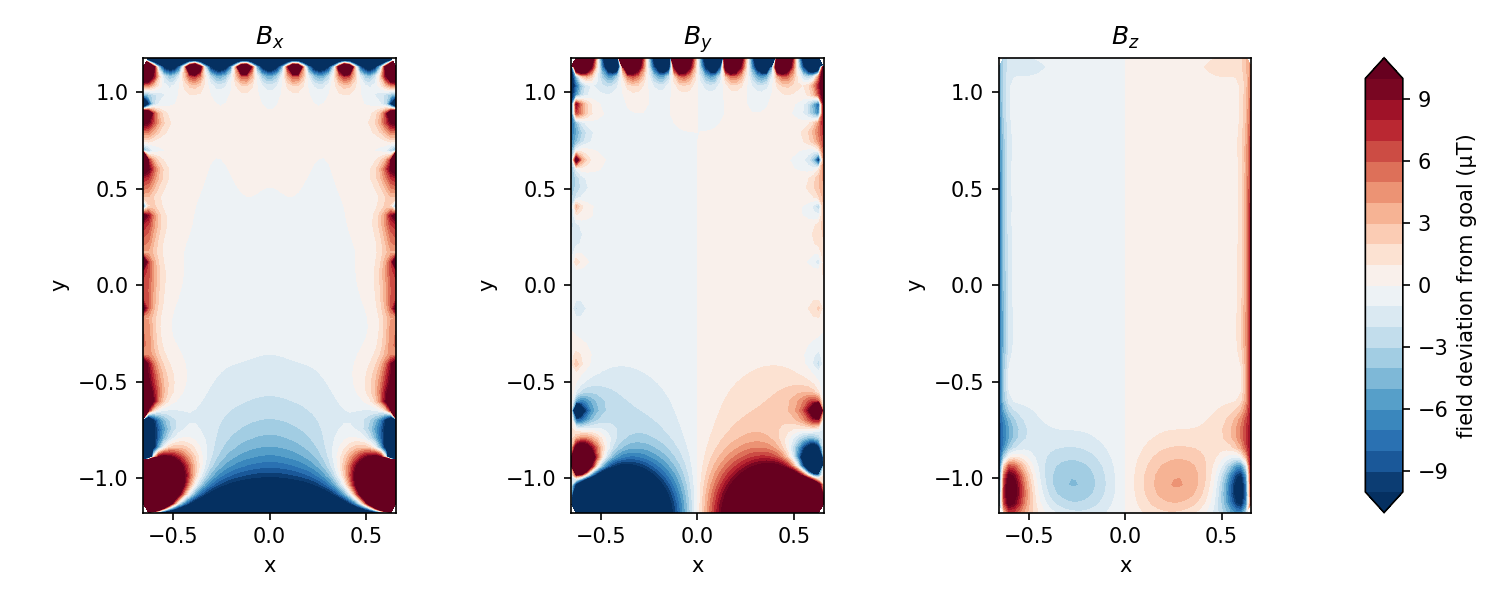
\includegraphics[width=\linewidth]{gfx/prototype/open_design_Xcoil_field_XY_z0_33.png}
  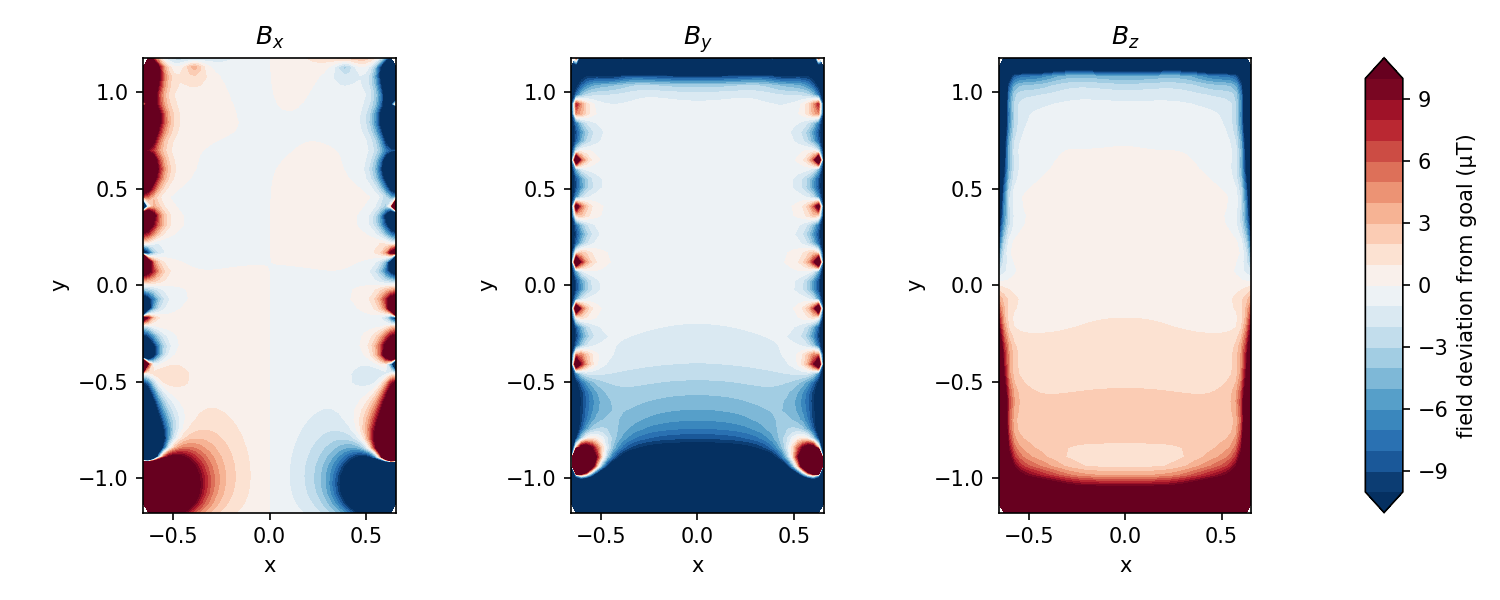
\includegraphics[width=\linewidth]{gfx/prototype/open_design_n8coil_field_XY_z0_33.png}
  \caption{Simulation of the open-design cage. The colour represents the deviation from the target field, for the $x$, $y$ and $z$ components of the field. Section in the XY plane at height $z=\SI{33}{\centi\meter}$ is shown. The open face is on the bottom of the plots. Top: coil designed to produce a homogeneous field along $x$ (left-to-right on the plot). Bottom: $n=8$ gradient (see some table somewhere)\ldots}
  \label{fig:prototype_open_design_simulation}
\end{figure}

\begin{figure}
  \centering
  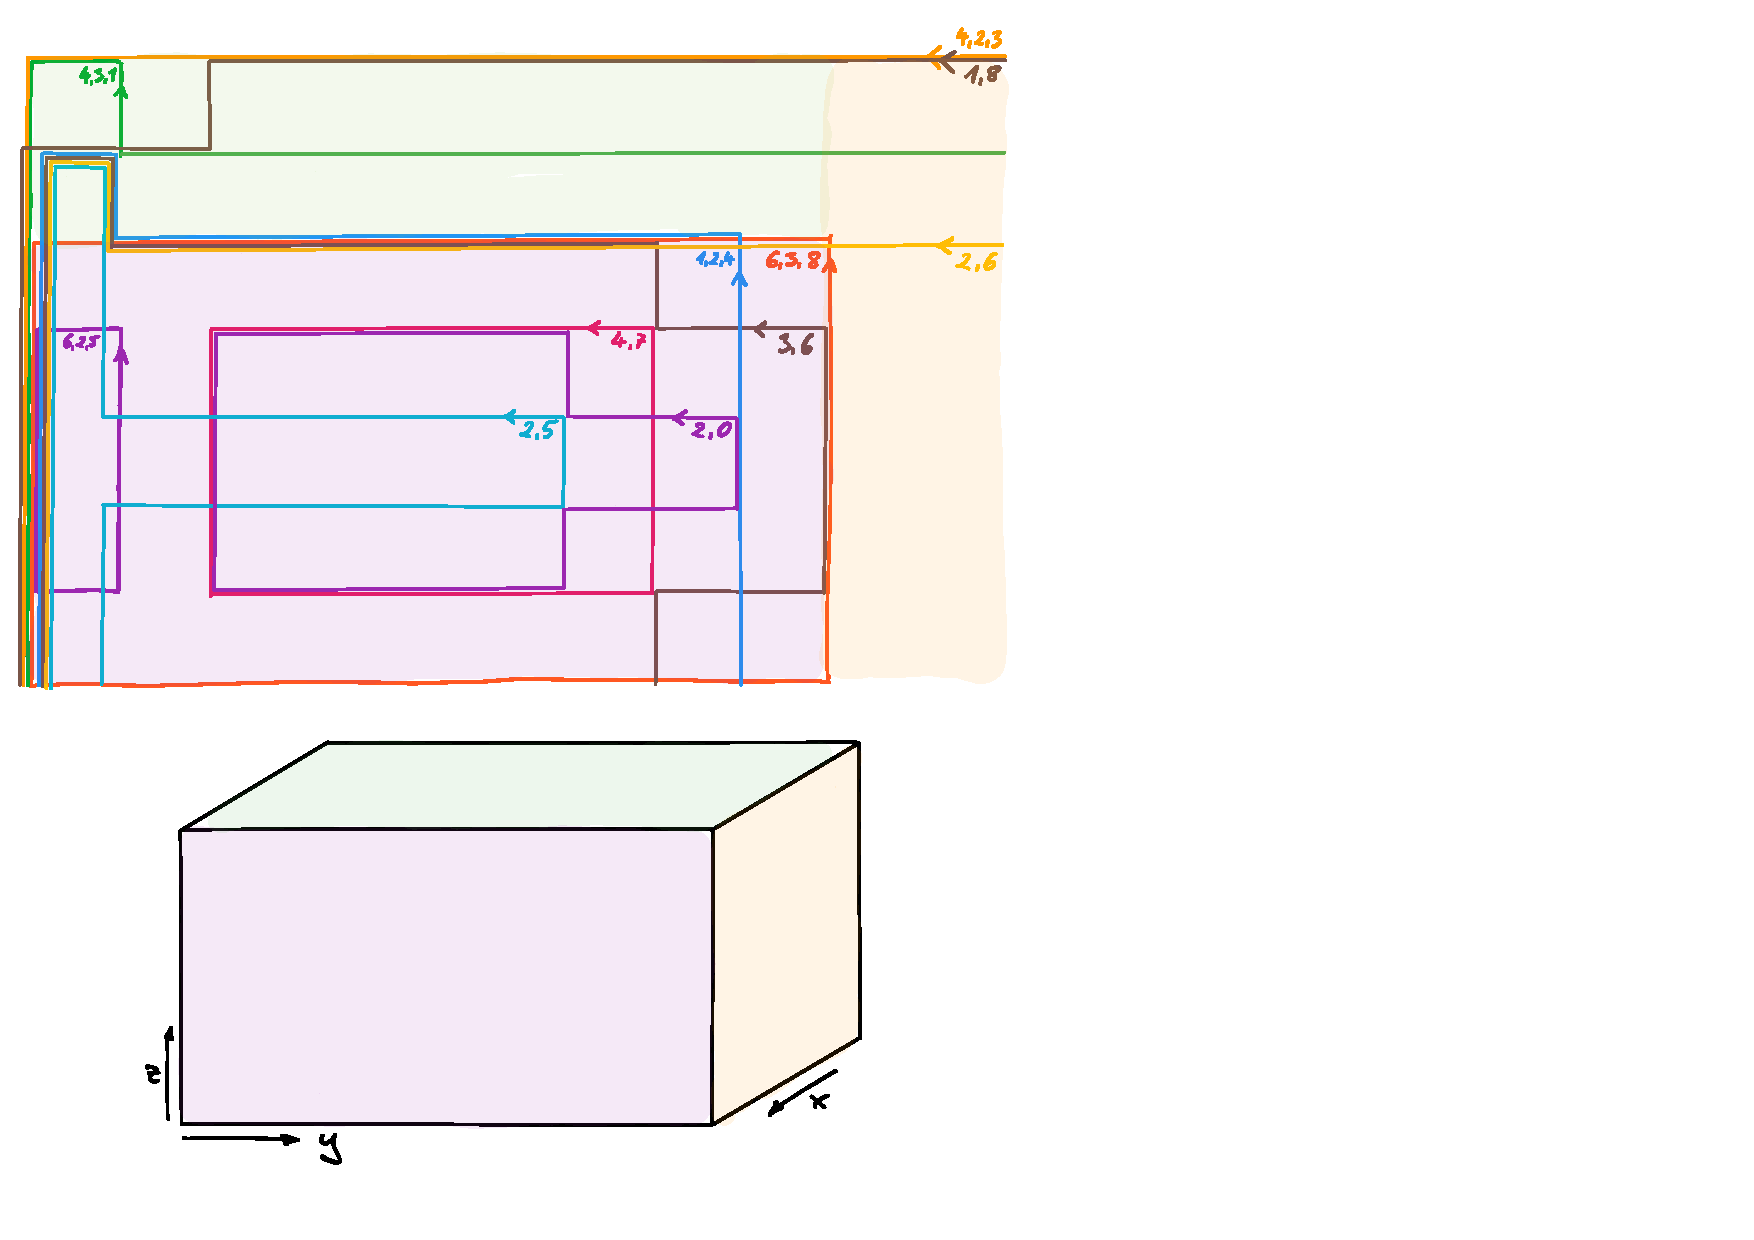
\includegraphics[width=\linewidth]{gfx/prototype/open_design_Xcoil_coils.pdf}
  \caption{X coils, first 22 coils, windings of 5A, 1A and 0.1A\ldots}
  \label{fig:prototype_open_design_Xcoil_coils}
\end{figure}

\begin{figure}
  \centering
  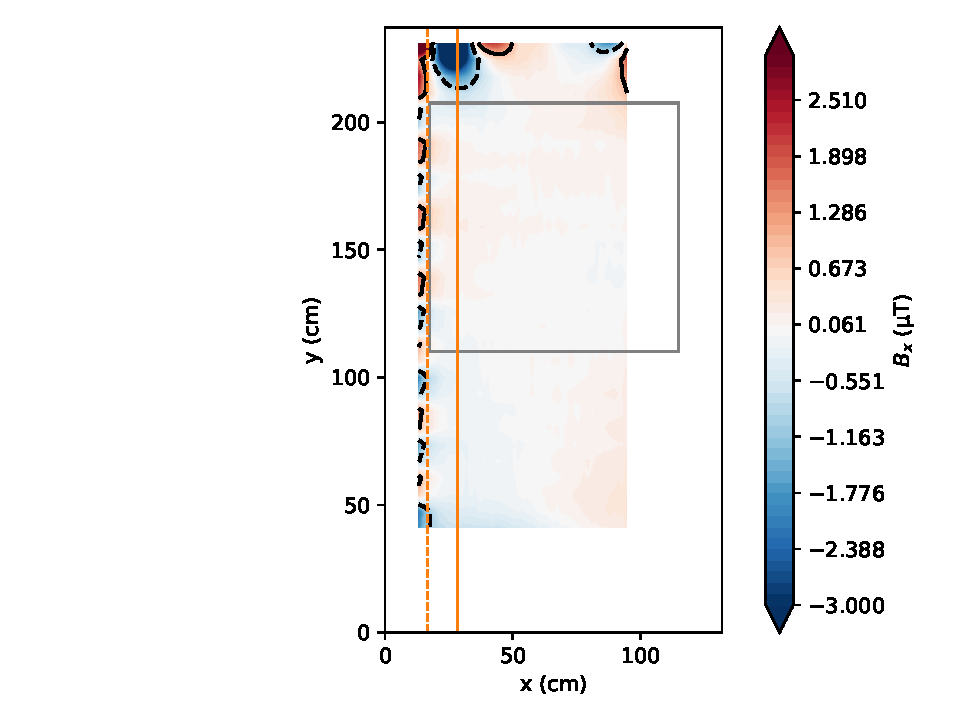
\includegraphics[width=0.45\linewidth,trim={5cm 0 0 0},clip]{gfx/prototype/open_planar_map_Y_Bx.pdf}\quad
  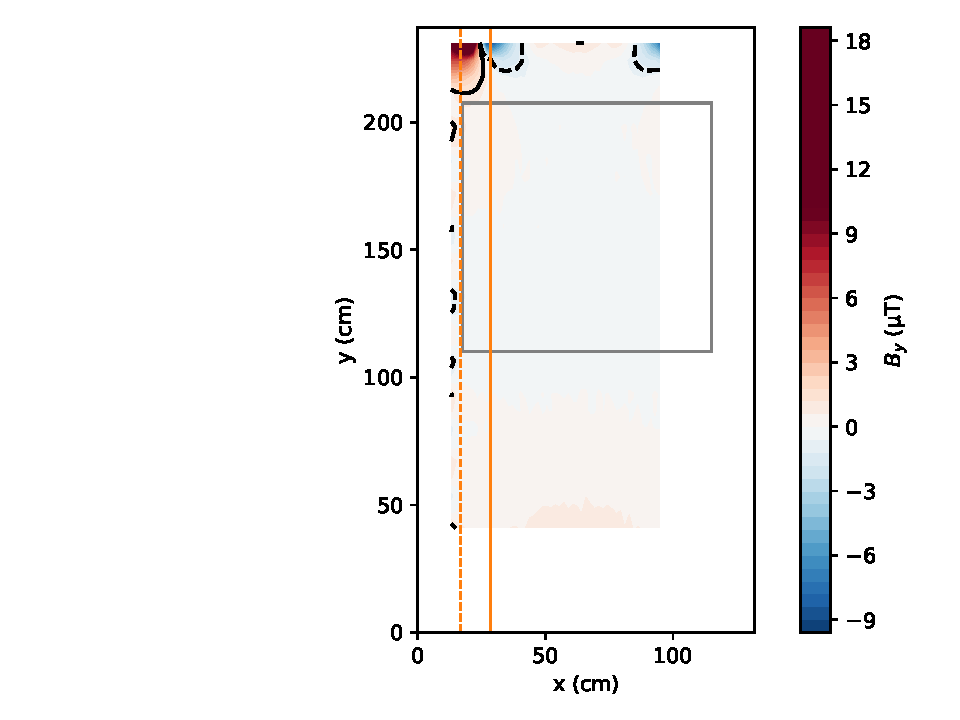
\includegraphics[width=0.45\linewidth,trim={5cm 0 0 0},clip]{gfx/prototype/open_planar_map_Y_By.pdf}
  \caption{Left: the $x$ component of the field. Right: the $y$ component, relative to the reference value of \SI{49.854}{\micro\tesla} as measured in the middle.}
  \label{fig:prototype_open_design_Ycoil_maps}
\end{figure}

\begin{figure}
  \centering
  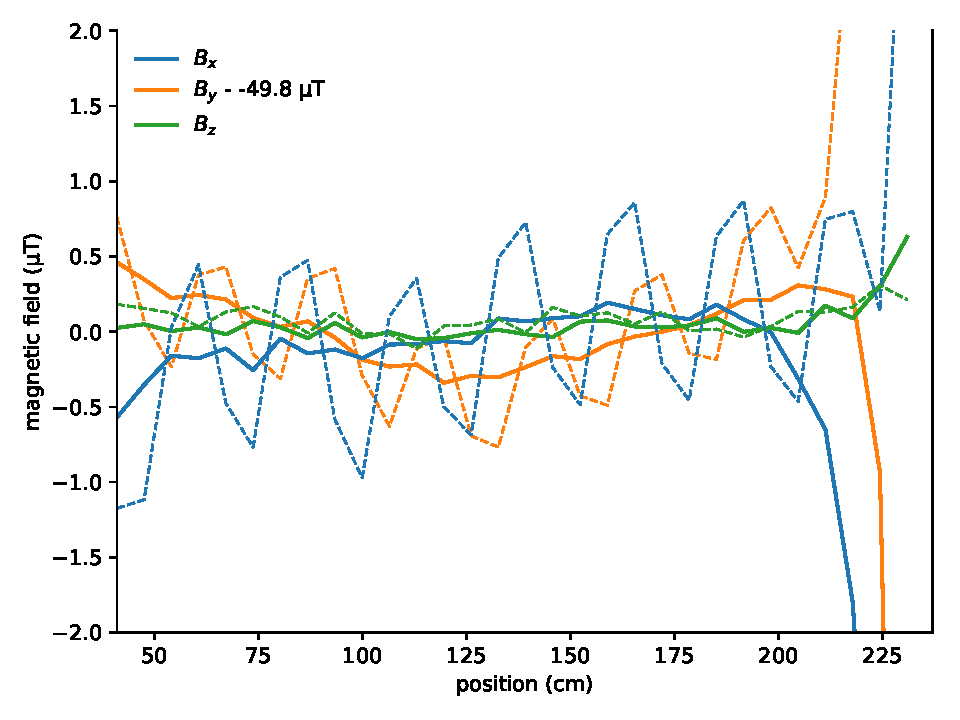
\includegraphics[width=0.7\linewidth]{gfx/prototype/open_planar_map_Y_By_section.pdf}
  \caption{\ldots}
  \label{fig:prototype_open_design_Ycoil_map_section}
\end{figure}

\section{n2EDM design}

\begin{figure}
  \centering
  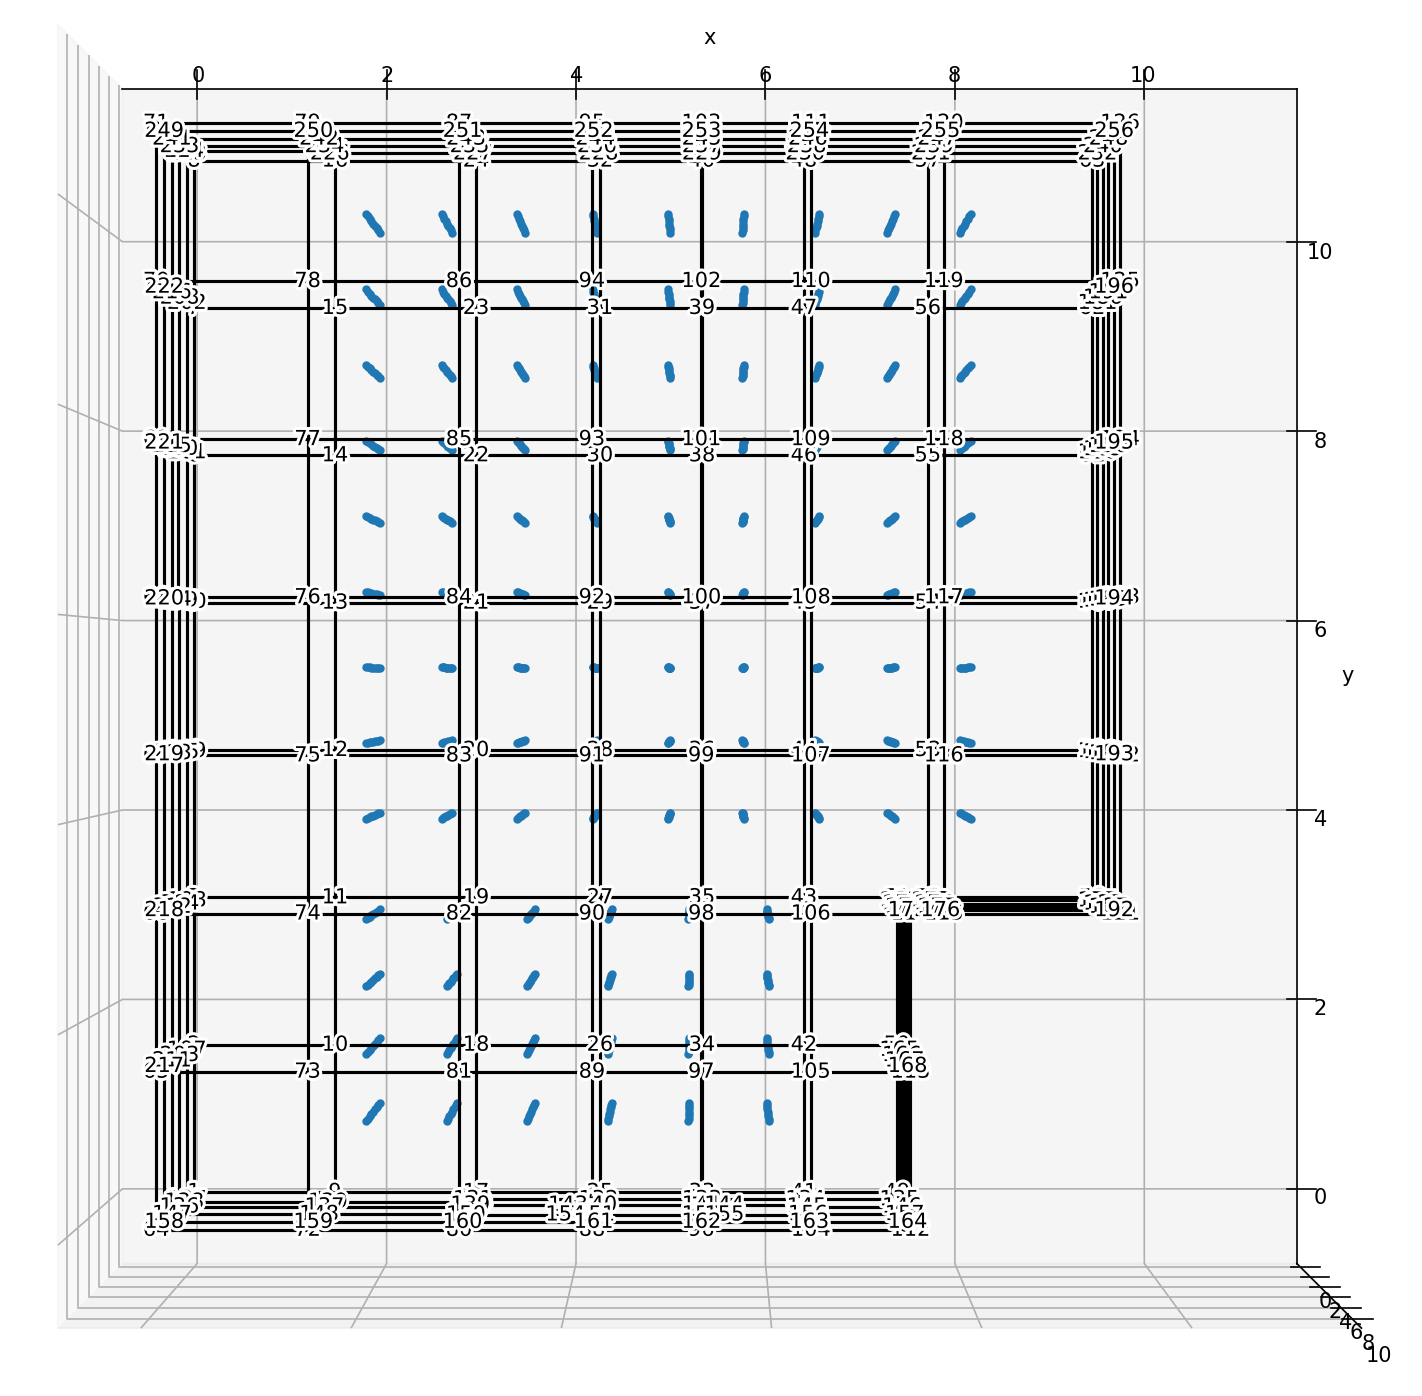
\includegraphics[width=\linewidth]{gfx/prototype/n2EDM_system_top.png}
  \caption{Replace with a better figure showing the design\ldots}
  \label{fig:prototype_open_design_Xcoil_coils}
\end{figure}

\begin{figure}
  \centering
  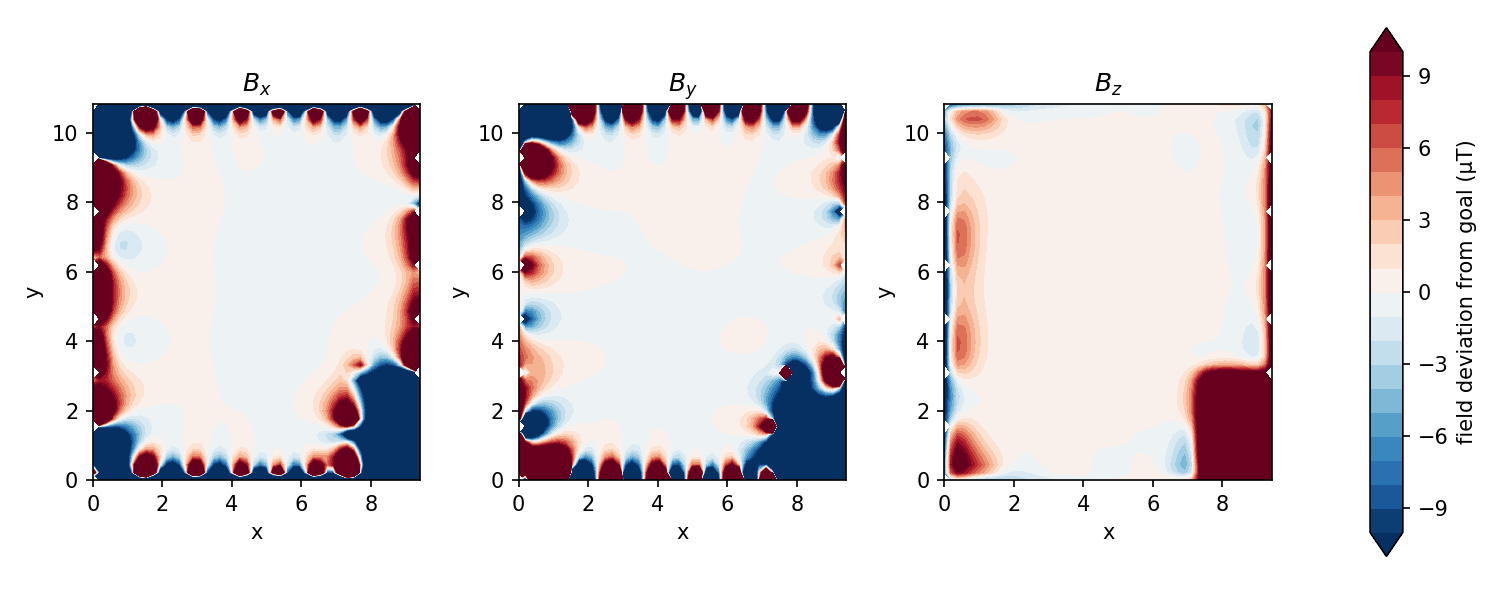
\includegraphics[width=\linewidth]{gfx/prototype/n2EDM_field_Xcoil_XY_z6_4.png}
  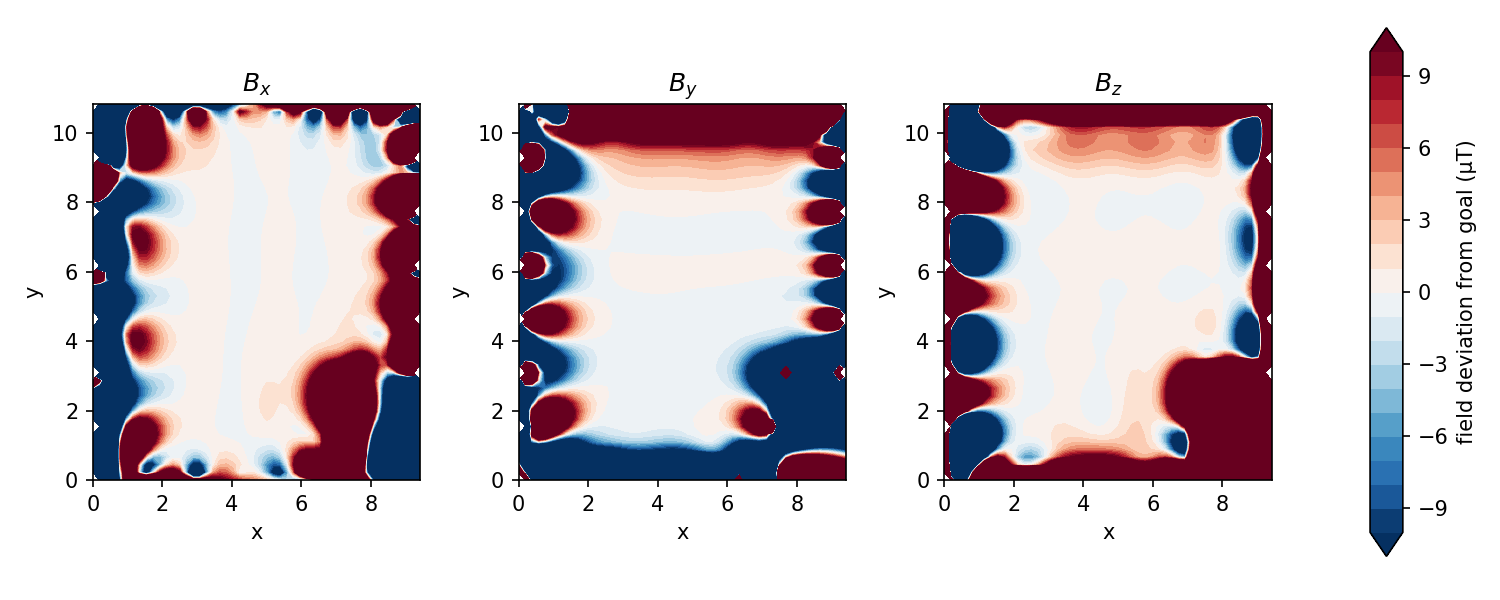
\includegraphics[width=\linewidth]{gfx/prototype/n2EDM_field_n6coil_XY_z6_4.png}
  \caption{Simulation of the n2EDM design. The colour represents the deviation from the target field, for the $x$, $y$ and $z$ components of the field. Section in the XY plane at height $z=\SI{6.4}{\meter}$ is shown. The open face is on the bottom of the plots. Top: coil designed to produce a homogeneous field along $x$ (left-to-right on the plot). Bottom: $n=6$ gradient (see some table somewhere)\ldots}
  \label{fig:prototype_open_design_simulation}
\end{figure}

The volume is cubic.

The SFC system is going to be very large --- $\unit[6x6x6]{m^3}$. Elaborate designs, such as wires of variable length, or arbitrarily bended wires would be complicated to realise in such scale.

Moreover, the system is going to enclose the whole apparatus.
Super crucial --- many coils on the same surface 3 for the first order compensation, but then 9 for gradients. That is already 12 coils. If one only restrict oneself to a surface, it is guaranteed to end up with it densely covered with wires. In this approach the geometry is limited by design.

Mention, that the \micro-metal presence does not disturb much, as it is already placed in a small field.


Design goals / challenges:
\begin{enumerate}
  \item Better shielding factor. Attenuation by a factor of 50 in the whole volume of the shield. The design goal has been set to reach at most 2\% of the ambient magnetic field in the
  whole volume of the experiment. In \unit[50]{\micro T} this corresponds to a nice value of \unit[1]{\micro T}.
  \item Very large fiducial volume --- due to spatial constrains of the experimental site --- biological shielding. PUT IMAGE!!! Not only is the compensation expected to be better, but also provide a much larger volume. Next version of the experiment --- much larger.
  \item As is nEDM --- many coil system. But orthogonal, or at least close to one. Three coils for compensating the three homogeneous components of the magnetic field. Then 9 for gradients. The strongest fields are low--order, and only these require strong compensation coils (thick wires, big and expensive power supplies). The higher--order coils may be constructed with thinner wires and cheaper power supplies.
  Additionally, this makes the control of the system simpler.
  This also states the problem better. One has to design and construct coils that create homogeneous field in the volume occupied by the shield. Maybe elaborate more on the field decomposition!
  \item Coil tailored for the specific magnetic environment of the n2EDM site. Coils tailored for nearby magnets.
\end{enumerate}
